\pdfminorversion=4\pdfobjcompresslevel=0
\documentclass[11pt,a4paper]{article}
\usepackage[T1]{fontenc}
\usepackage{mathpazo}
\usepackage[scaled=0.95]{helvet}
\usepackage[margin=2.2cm,top=2.4cm,bottom=2.2cm,headheight=15pt]{geometry}
\usepackage{graphicx,xcolor,amsmath,amssymb,booktabs,array,enumitem,fancyhdr,caption,subcaption,float,pifont,lastpage,needspace,microtype,url,tcolorbox}
\usepackage[colorlinks=true,urlcolor=teal,linkcolor=teal]{hyperref}
\tcbuselibrary{skins,breakable}
\definecolor{teal}{RGB}{0,98,112}
\definecolor{amber}{RGB}{226,140,0}
\definecolor{mist}{RGB}{233,244,245}
\definecolor{sand}{RGB}{253,246,232}
\definecolor{ink}{RGB}{38,50,56}
\color{ink}
\setlength{\parindent}{0pt}\setlength{\parskip}{4pt}
\renewcommand{\arraystretch}{1.18}
\setlist[itemize]{label=\textcolor{amber}{\textbullet},leftmargin=1.3em,itemsep=2pt,topsep=2pt,parsep=0pt}
\captionsetup{font={sf,small},labelfont={sf,bf,color=teal},labelsep=period,skip=4pt}
\captionsetup[table]{position=bottom}
\pagestyle{fancy}\fancyhf{}
\fancyhead[L]{\sffamily\small\color{teal}\textbf{EC2L104} \textcolor{gray}{\textbar} Discrete CMOS Inverter Board}
\fancyhead[R]{\sffamily\small\color{gray}Chemitiganti Siva Sai \textbar\ 25EC01002}
\fancyfoot[C]{\sffamily\small\color{gray}Page \thepage\ of \pageref{LastPage}}
\renewcommand{\headrulewidth}{0.5pt}\renewcommand{\headrule}{\hbox to\headwidth{\color{teal}\leaders\hrule height \headrulewidth\hfill}}
\newcommand{\ok}{\textcolor{teal}{\ding{51}}}
\newcommand{\exhead}[2]{\Needspace{8\baselineskip}\vspace{8pt}\begin{tcolorbox}[enhanced,colback=teal,colframe=teal,arc=2pt,boxrule=0pt,left=8pt,right=8pt,top=3pt,bottom=3pt]\sffamily\bfseries\color{white}\large #1 \hfill{\normalsize\bfseries #2}\end{tcolorbox}\vspace{-2pt}}
\newcommand{\lab}[2]{\Needspace{5\baselineskip}\vspace{6pt}{\sffamily\bfseries\color{teal}\large #1}\ {\sffamily\bfseries\color{ink}#2}\par\vspace{-2pt}{\color{amber}\rule{2.2em}{1.4pt}}\par\vspace{2pt}}
\newtcolorbox{answer}{enhanced,breakable,colback=mist,colframe=mist,boxrule=0pt,arc=2pt,left=8pt,right=6pt,top=3pt,bottom=3pt,borderline west={3pt}{0pt}{teal},before skip=6pt,after skip=8pt,title={\sffamily\bfseries\small\color{teal}ANSWER},coltitle=teal,colbacktitle=mist,attach boxed title to top left={yshift=-1pt},boxed title style={colback=mist,boxrule=0pt,top=0pt,bottom=0pt,left=0pt}}
\newtcolorbox{keybox}[1]{enhanced,colback=sand,colframe=amber!70,boxrule=0.6pt,arc=2pt,left=8pt,right=8pt,top=4pt,bottom=4pt,title={\sffamily\bfseries\small #1},coltitle=ink,colbacktitle=amber!35,fonttitle=\sffamily}
\newcommand{\tablehead}[1]{\rowcolor{teal}\color{white}\sffamily\bfseries #1}
\usepackage{colortbl}

\emergencystretch=2em
\begin{document}
%------------------------------------------------------------ COVER
\begin{tcolorbox}[enhanced,colback=teal,colframe=teal,arc=3pt,boxrule=0pt,left=16pt,right=16pt,top=10pt,bottom=10pt]
\raggedright
{\sffamily\color{amber}\bfseries\small EC2L104 \textbar\ INTRODUCTION TO EDA TOOLS \textbar\ MODULE 10}\par
\vspace{4pt}{\color{amber}\rule{\linewidth}{0.8pt}}\par\vspace{6pt}
{\sffamily\bfseries\color{white}\fontsize{26}{32}\selectfont From Circuit to Board:\par A Discrete CMOS Inverter\par}
\vspace{6pt}{\color{white!45!teal}\rule{\linewidth}{0.5pt}}\par\vspace{5pt}
{\sffamily\color{white}\large LTspice $\rightarrow$ KiCad schematic $\rightarrow$ PCB layout $\rightarrow$ Gerber files\par}
\end{tcolorbox}
\vspace{8pt}
\begin{tabular}{@{\hspace{4pt}}>{\sffamily\bfseries\color{teal}}l@{\hspace{1.6em}}l@{}}
Name & Chemitiganti Siva Sai\\
Roll number & 25EC01002 \quad (project \texttt{25EC01002\_INV})\\
Circuit & 2N7000 (NMOS) + BS250 (PMOS), $V_{DD}=5$ V, $R_1=1\,\mathrm{k}\Omega$, LED indicator\\
GitHub & {\small\url{https://github.com/ChemitigantiSivaSai/25EC01002_PCB_Design}}\\
Date & 15-11-2026\\
\end{tabular}

\vspace{6pt}
\begin{keybox}{RESULTS AT A GLANCE}
\small\sffamily
\begin{tabular}{@{}>{\raggedright\arraybackslash}p{4.0cm}>{\raggedright\arraybackslash}p{3.9cm}>{\raggedright\arraybackslash}p{3.4cm}>{\raggedright\arraybackslash}p{3.1cm}@{}}
\textbf{Switching threshold} $V_M$ & \mbox{2.35 V (5 V), 4.07 V (9 V)} & \textbf{LED current} (sim.) & 4.25 mA\\
\textbf{Output levels} & 4.94 V / $\approx$ 0 V & \textbf{ERC} & 0 errors, 0 warnings\\
\textbf{Dead zone at 5 V} & None & \textbf{DRC} & 0 / 0 / 0\\
\textbf{Board} & 50 $\times$ 40 mm, 2-layer & \textbf{+5V track resistance} & 0.028 $\Omega$ (47.1 mm)\\
\textbf{Exercise 5} & options 1, 2, 3, 4 done & \textbf{Buffer (option 1)} & $V_M$ 2.415 V, DRC 0 / 0 / 0\\
\end{tabular}
\end{keybox}

%------------------------------------------------------------ EX 0
\exhead{Exercise 0}{Pre-KiCad: simulate before you build (LTspice)}
\lab{L1}{Build the inverter in LTspice}
\begin{itemize}
\item Circuit: 2N7000 (pull-down) and BS250 (pull-up), gates joined to $V_{IN}$, drains joined at \texttt{out}, then $R_1=1\,\mathrm{k}\Omega$ and LED \texttt{D1} to ground.
\item Models: \texttt{2N7000.onsemi.lib}, \texttt{BS250.philips.lib} (manufacturer SPICE models), \texttt{.include}d from the project folder.
\item $V_{DD}=5$ V; $V_{IN}$ swept 0--5 V for \texttt{.dc}, and \texttt{PULSE(0 5 0 0 0 0.5ms 1ms 3)} for \texttt{.tran}.
\item Note: D1 resolves to the default diode (\texttt{.model D D}), not the \texttt{LED} line, so its drop is 0.69 V.
\end{itemize}
\begin{figure}[H]\centering
\begin{subfigure}{0.49\linewidth}\centering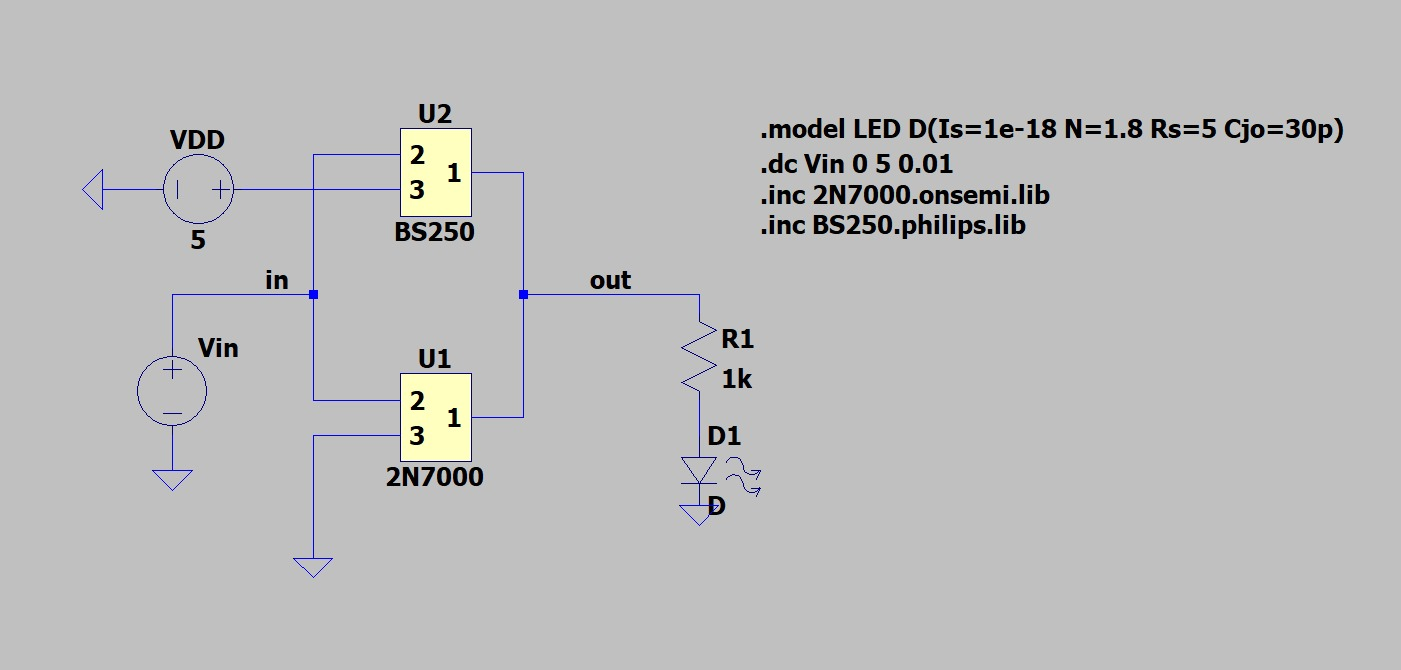
\includegraphics[width=\linewidth]{figures/l1-dc.png}\caption{DC sweep circuit}\end{subfigure}\hfill
\begin{subfigure}{0.49\linewidth}\centering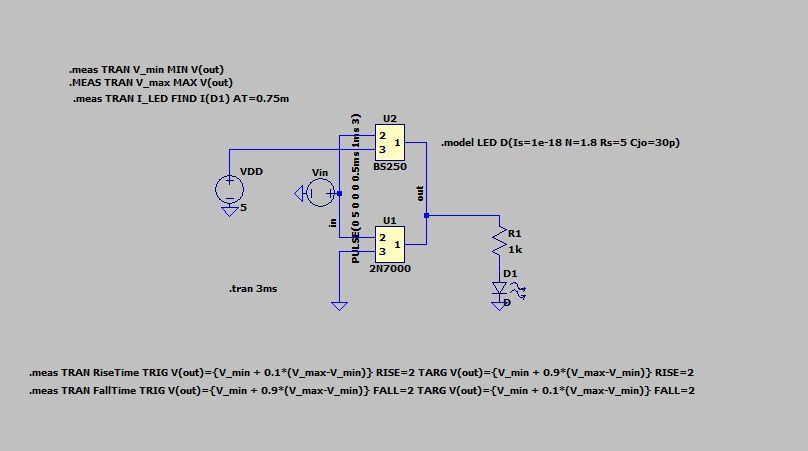
\includegraphics[width=\linewidth]{figures/l1-tran.png}\caption{Transient circuit}\end{subfigure}
\caption{LTspice schematics with model names visible.}\end{figure}

\lab{L2}{Voltage transfer curve}
\begin{itemize}
\item Run: \texttt{.dc Vin 0 5 0.01}.
\item Switching threshold: $V_M=\mathbf{2.35}$ V (where $V_{OUT}=V_{DD}/2=2.5$ V).
\item Output levels: $V_{OH}=4.94$ V, $V_{OL}\approx0$ V; the transition is sharp (about 0.2 V wide).
\item Dead zone at 5 V: \textbf{none}; both devices conduct for 2.24 V $<V_{IN}<$ 2.70 V.
\item $V_{DD}=9$ V: $V_M=\mathbf{4.07}$ V; still no dead zone (both conduct for 2.24 V to 6.70 V).
\end{itemize}
\begin{figure}[H]\centering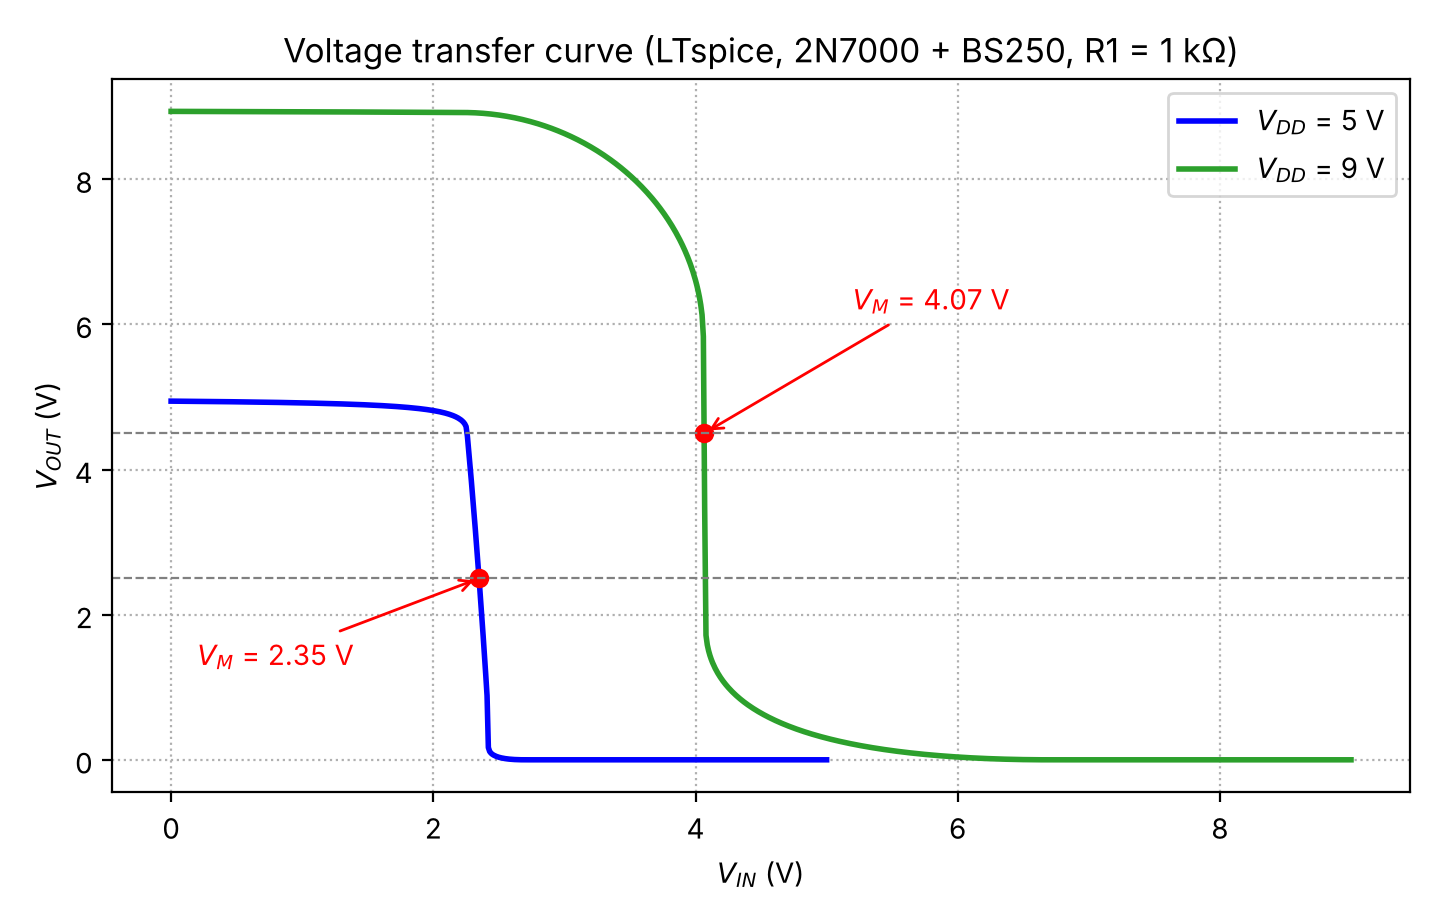
\includegraphics[width=0.74\linewidth]{figures/l2-vtc.png}\caption{VTC with $V_M$ marked for $V_{DD}=5$ V and 9 V.}\end{figure}
\begin{answer}
\begin{itemize}
\item A dead zone needs $V_{TN}+|V_{TP}|>V_{DD}$: here $2.236+2.3=4.54$ V $<5$ V, so there is none.
\item Higher $V_{DD}$ shifts $V_M$ up (2.35 V $\to$ 4.07 V) and widens the both-on window, so shoot-through current increases.
\item Datasheet worst cases (3 V and 3.5 V, sum 6.5 V) could create a dead zone at 5 V on real parts.
\end{itemize}
\end{answer}

\lab{L3}{LED current and transient}
\begin{itemize}
\item Simulated $I_{LED}$ at $V_{IN}=0$ V: \textbf{4.25 mA}.
\item Hand calculation: $(V_{DD}-V_F)/R_1=(5-0.69)/1\,\mathrm{k}\Omega=\mathbf{4.31}$ mA, with $V_F=0.69$ V from the simulation.
\item Difference: \textbf{1.3 \%}, caused by the 57 mV drop across the PMOS.
\item $t_r$ and $t_f$ come from the 10--90 \% \texttt{.meas} statements below.
\end{itemize}
{\footnotesize\ttfamily\raggedright\setlength{\parskip}{1pt}
.meas TRAN V\_min MIN V(out) \quad .MEAS TRAN V\_max MAX V(out)\par
\hangindent=1.5em .meas TRAN RiseTime TRIG V(out)=\{V\_min+0.1*(V\_max-V\_min)\} RISE=2 TARG V(out)=\{V\_min+0.9*(V\_max-V\_min)\} RISE=2\par
\hangindent=1.5em .meas TRAN FallTime TRIG V(out)=\{V\_min+0.9*(V\_max-V\_min)\} FALL=2 TARG V(out)=\{V\_min+0.1*(V\_max-V\_min)\} FALL=2\par}
\begin{table}[H]\centering\small\sffamily
\begin{tabular}{@{}lcc@{}}\rowcolor{teal}\color{white}\textbf{Quantity}&\color{white}\textbf{Value}&\color{white}\textbf{Unit}\\
$V_M$&2.35&V\\ \rowcolor{mist}$I_{LED}$&4.25&mA\\ $t_r$ (10--90 \%)&1.61&$\mu$s\\ \rowcolor{mist}$t_f$ (90--10 \%)&1.87&$\mu$s\\\end{tabular}
\caption{Simulation summary.}\end{table}
\begin{itemize}\small
\item LTspice limited the zero-time input edges to 50 $\mu$s, so $t_r$ and $t_f$ reflect that slow ramp, not the gates' intrinsic speed.
\end{itemize}
\begin{figure}[H]\centering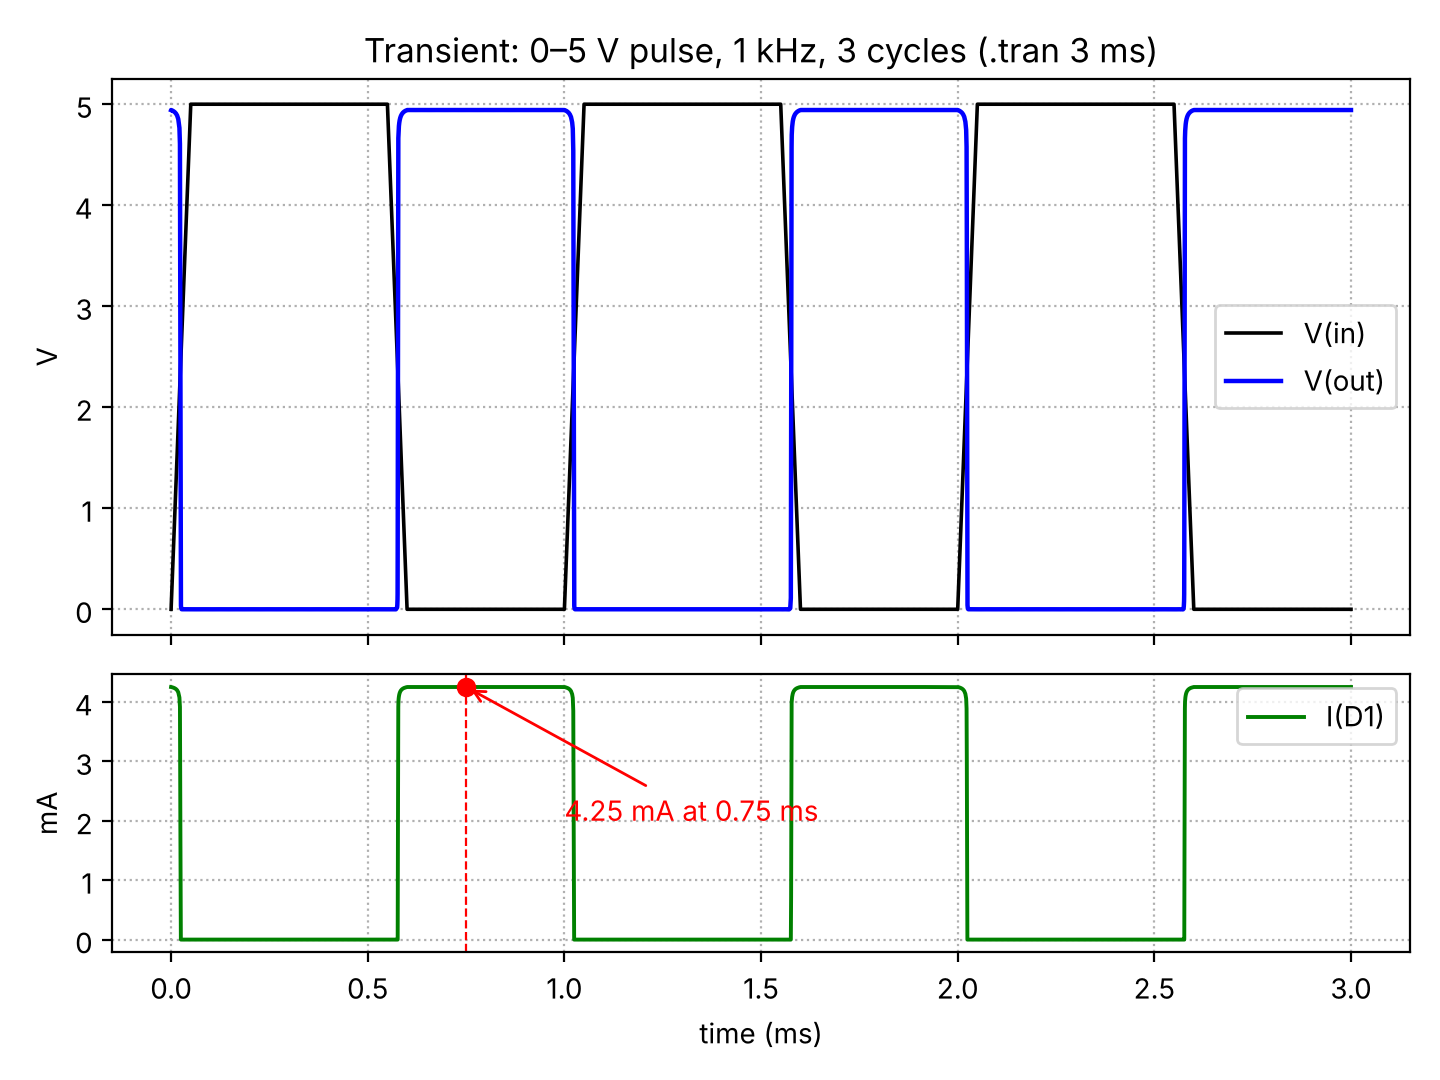
\includegraphics[width=0.74\linewidth]{figures/l3-transient.png}\caption{Transient response to the 0--5 V, 1 kHz pulse.}\end{figure}

\lab{L4}{Python plot}
\begin{itemize}
\item Script: \texttt{L4.py}
\item Plot has labelled axes, grid and $V_M=2.349$ V marked; saved at 300 dpi.
\item Commit link: \url{https://github.com/ChemitigantiSivaSai/KICAD.git}
\end{itemize}
\begin{figure}[H]\centering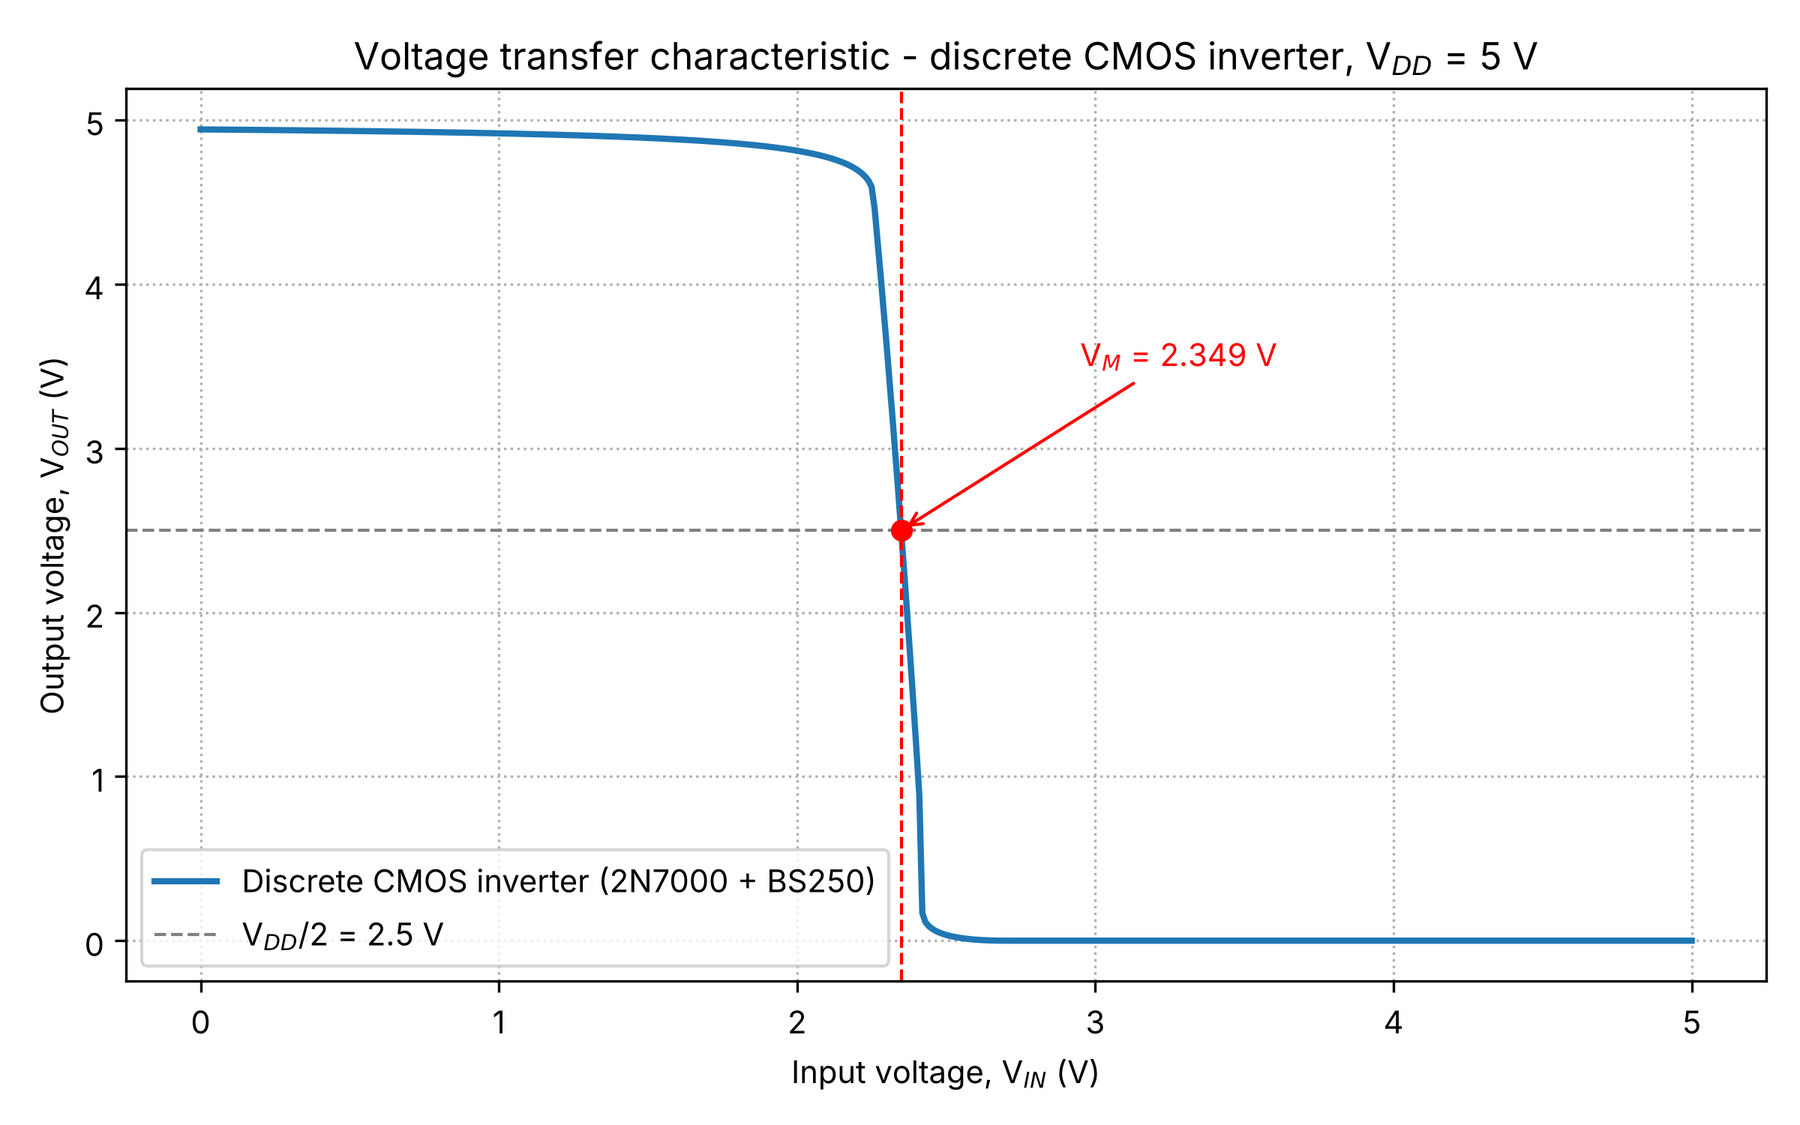
\includegraphics[width=0.66\linewidth]{figures/l4-vtc-python.png}\caption{VTC reproduced in Python (300 dpi).}\end{figure}

\lab{L5}{Comparison with 65 nm}
\begin{figure}[H]\centering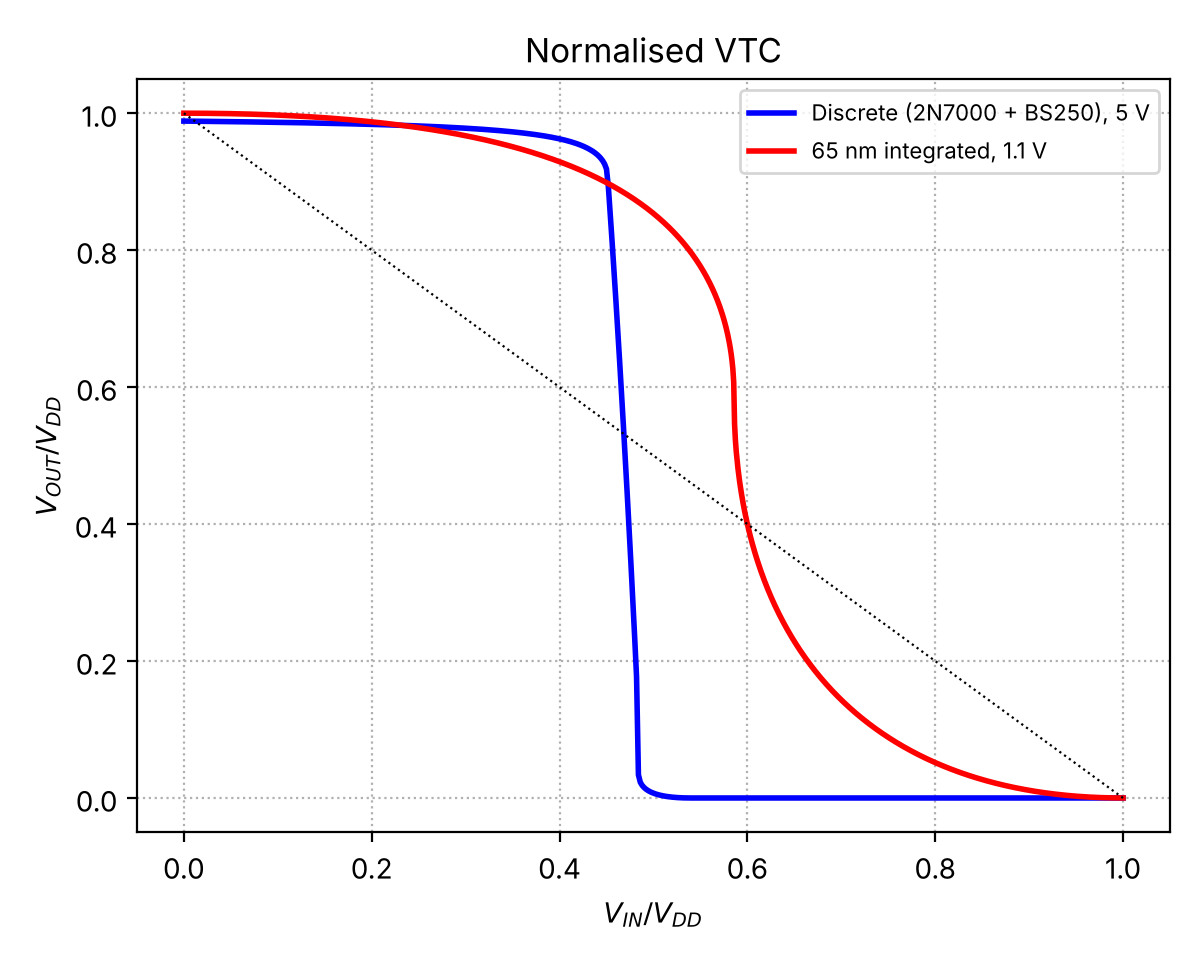
\includegraphics[width=0.5\linewidth]{figures/l5-overlay.png}\caption{Normalised VTC: $V_{OUT}/V_{DD}$ against $V_{IN}/V_{DD}$.}\end{figure}
\begin{answer}
\begin{itemize}
\item Shape: the discrete inverter switches abruptly (90 \% to 10 \% of $V_{DD}$ in 3 \% of $V_{DD}$ of input) because long-channel devices have little channel-length modulation, while the 65 nm inverter's short-channel effects spread the transition over about 29 \%.
\item Position: $V_M/V_{DD}=0.47$ (NMOS stronger) against 0.59 (PMOS stronger) because of different relative drive strengths.
\end{itemize}
\end{answer}

%------------------------------------------------------------ EX 1
\exhead{Exercise 1}{Schematic capture and ERC}
\begin{itemize}
\item Project \texttt{25EC01002\_INV}; file \texttt{25EC01002\_INV.kicad\_sch}.
\item \ok\ Eight symbols placed \quad \ok\ Q2 flipped (source to +5V) \quad \ok\ +5V, GND and 2$\times$PWR\_FLAG
\item \ok\ POT\_W and VIN labelled and brought to J2 \quad \ok\ Annotated
\item ERC result: \textbf{0 errors, 0 warnings}.
\end{itemize}
\begin{figure}[H]\centering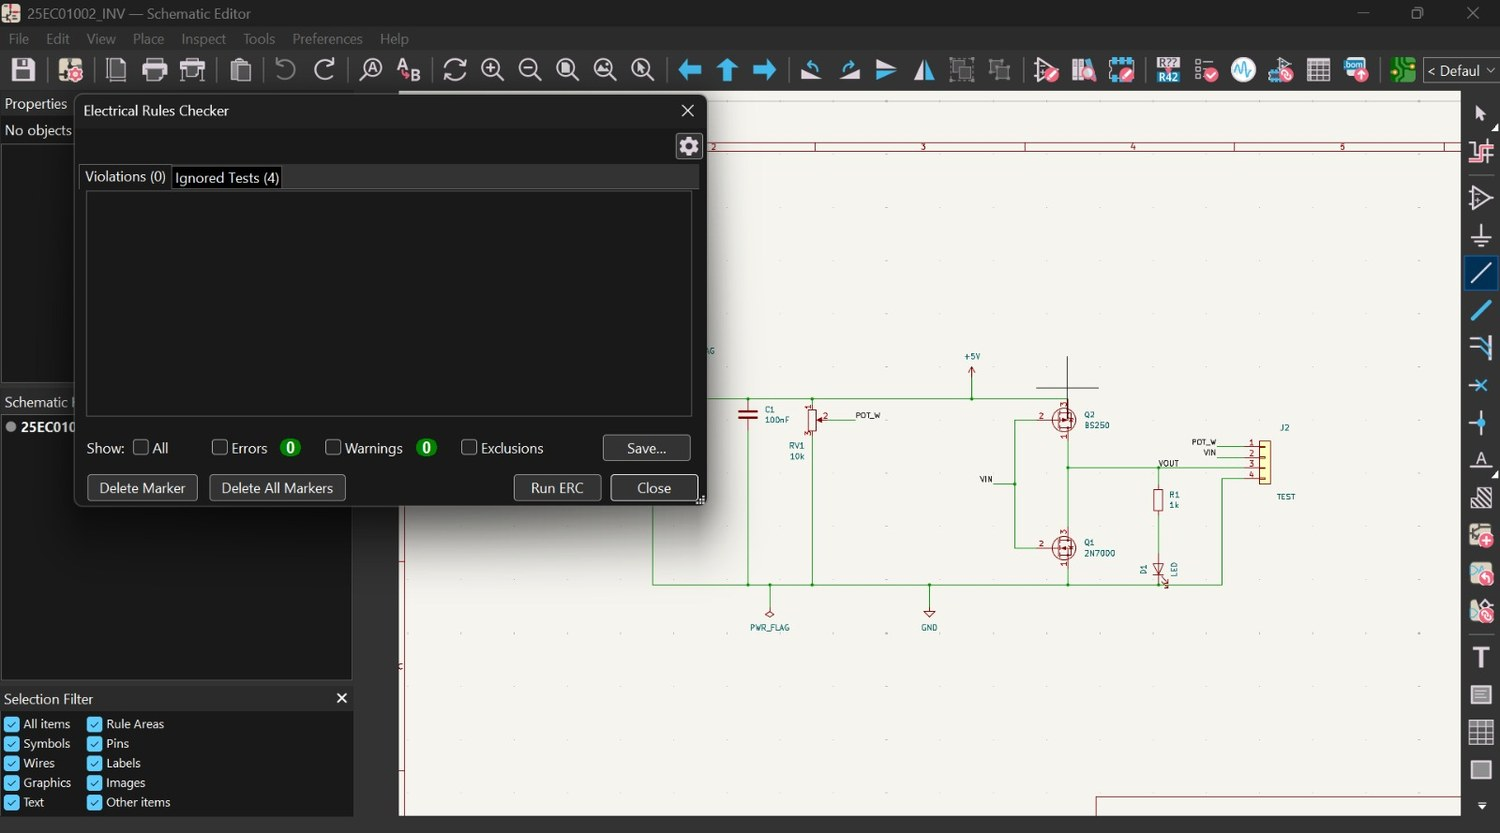
\includegraphics[width=0.82\linewidth]{figures/e1-erc.jpg}\caption{ERC dialog: 0 errors, 0 warnings.}\end{figure}
\begin{answer}
\textbf{Why a PWR\_FLAG?}
\begin{itemize}
\item +5V and GND enter through the passive pins of connector J1, so no pin is a power output.
\item The ERC then reports ``power input pin not driven''; PWR\_FLAG declares the net as externally supplied, with no change to the netlist.
\end{itemize}
\textbf{With an on-board regulator:}
\begin{itemize}
\item The regulator output is a power-output pin, so the flag on +5V is no longer needed.
\item The input and ground rails still enter from the connector and keep their flags.
\end{itemize}
\end{answer}

%------------------------------------------------------------ EX 2
\exhead{Exercise 2}{Footprints}
\begin{itemize}
\item Parts: 2N7000 and BS250; datasheets: Vishay Siliconix 70226 and 70209.
\item Footprints assigned (8), all through-hole; Q1 and Q2 use \texttt{TO-92\_Inline}.
\item Netlist update (F8): \textbf{0 warnings, 0 errors}.
\end{itemize}
\begin{table}[H]\centering\small\sffamily
\begin{tabular}{@{}llccc@{}}\rowcolor{teal}\color{white}\textbf{Part}&\color{white}\textbf{Pin}&\color{white}\textbf{KiCad symbol}&\color{white}\textbf{Datasheet lead}&\color{white}\textbf{Agree?}\\
Q1 2N7000&1&S&S&\ok\\ Q1 2N7000&2&G&G&\ok\\ Q1 2N7000&3&D&D&\ok\\
\rowcolor{mist}Q2 BS250&1&D&D&\ok\\ \rowcolor{mist}Q2 BS250&2&G&G&\ok\\ \rowcolor{mist}Q2 BS250&3&S&S&\ok\\\end{tabular}
\caption{Symbol pins against datasheet leads.}\end{table}
\begin{answer}
\begin{itemize}
\item Both parts agree with their symbols (2N7000: S-G-D; BS250: D-G-S), so no change is needed.
\item If one did not agree, on a fabricated board: (1) cross the outer leads or use a small adapter; (2) cut the two tracks and solder jumper wires swapping drain and source.
\end{itemize}
\end{answer}

%------------------------------------------------------------ EX 3
\exhead{Exercise 3}{Layout, routing and DRC}
\begin{itemize}
\item \ok\ 50 $\times$ 40 mm outline on Edge.Cuts \quad \ok\ four M3 holes, 4 mm from corners, ``Not in schematic''
\item \ok\ Power net class (+5V, GND) \quad \ok\ GND pour on B.Cu with thermal reliefs \quad \ok\ silkscreen $\geq1$ mm inside
\item Rules: signal tracks \textbf{0.25 mm}, power \textbf{0.8 mm}, clearance \textbf{0.2 mm}, via \textbf{0.6 mm} (none used).
\item DRC: \textbf{0 violations, 0 unconnected items, 0 schematic-parity errors}.
\end{itemize}
\begin{figure}[H]\centering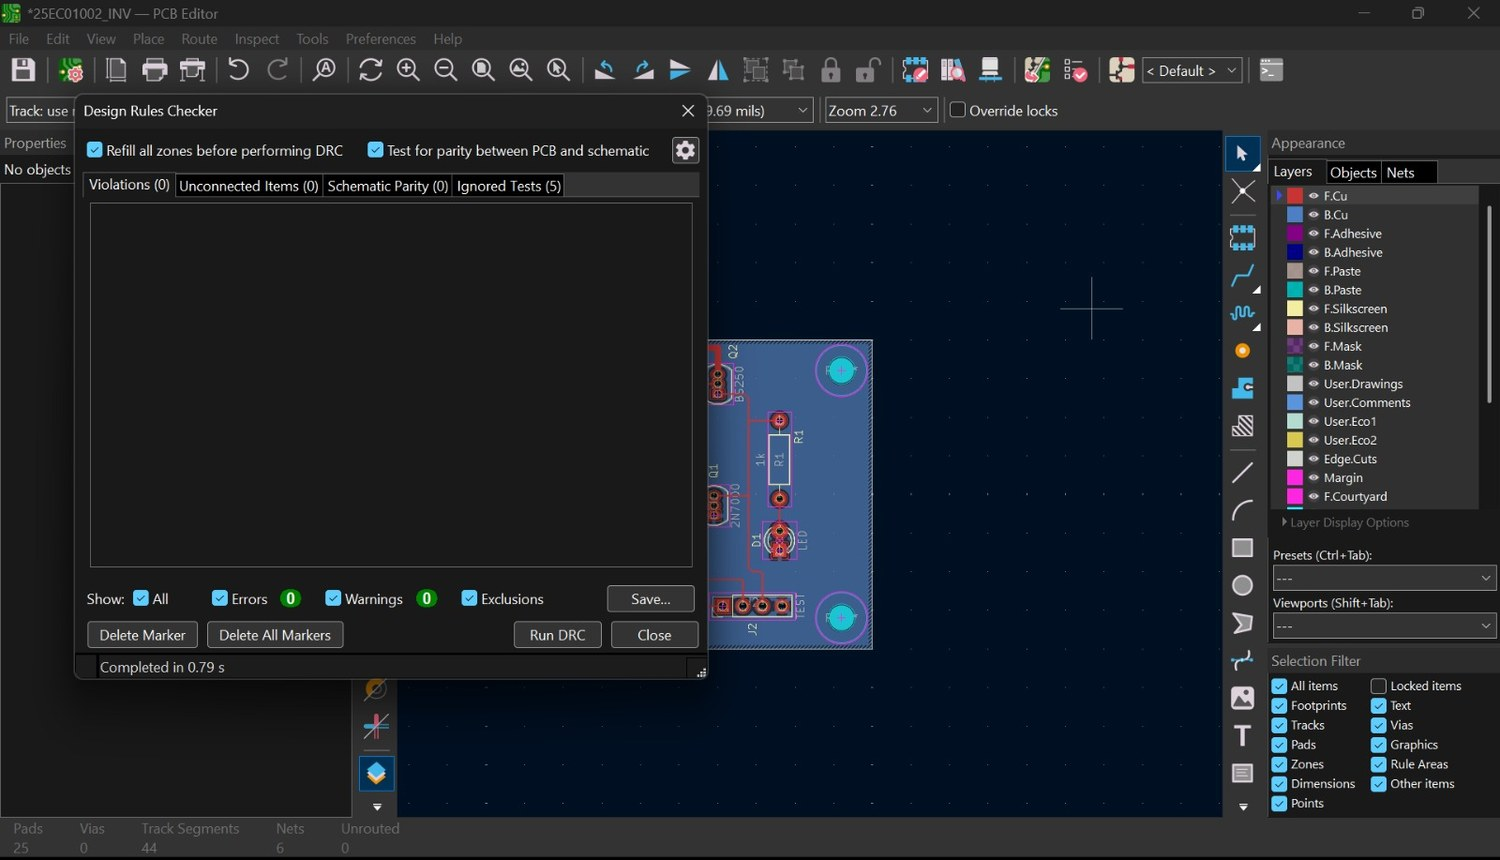
\includegraphics[width=0.84\linewidth]{figures/e3-drc.jpg}\caption{DRC dialog: Violations, Unconnected Items and Schematic Parity all 0.}\end{figure}
\begin{figure}[H]\centering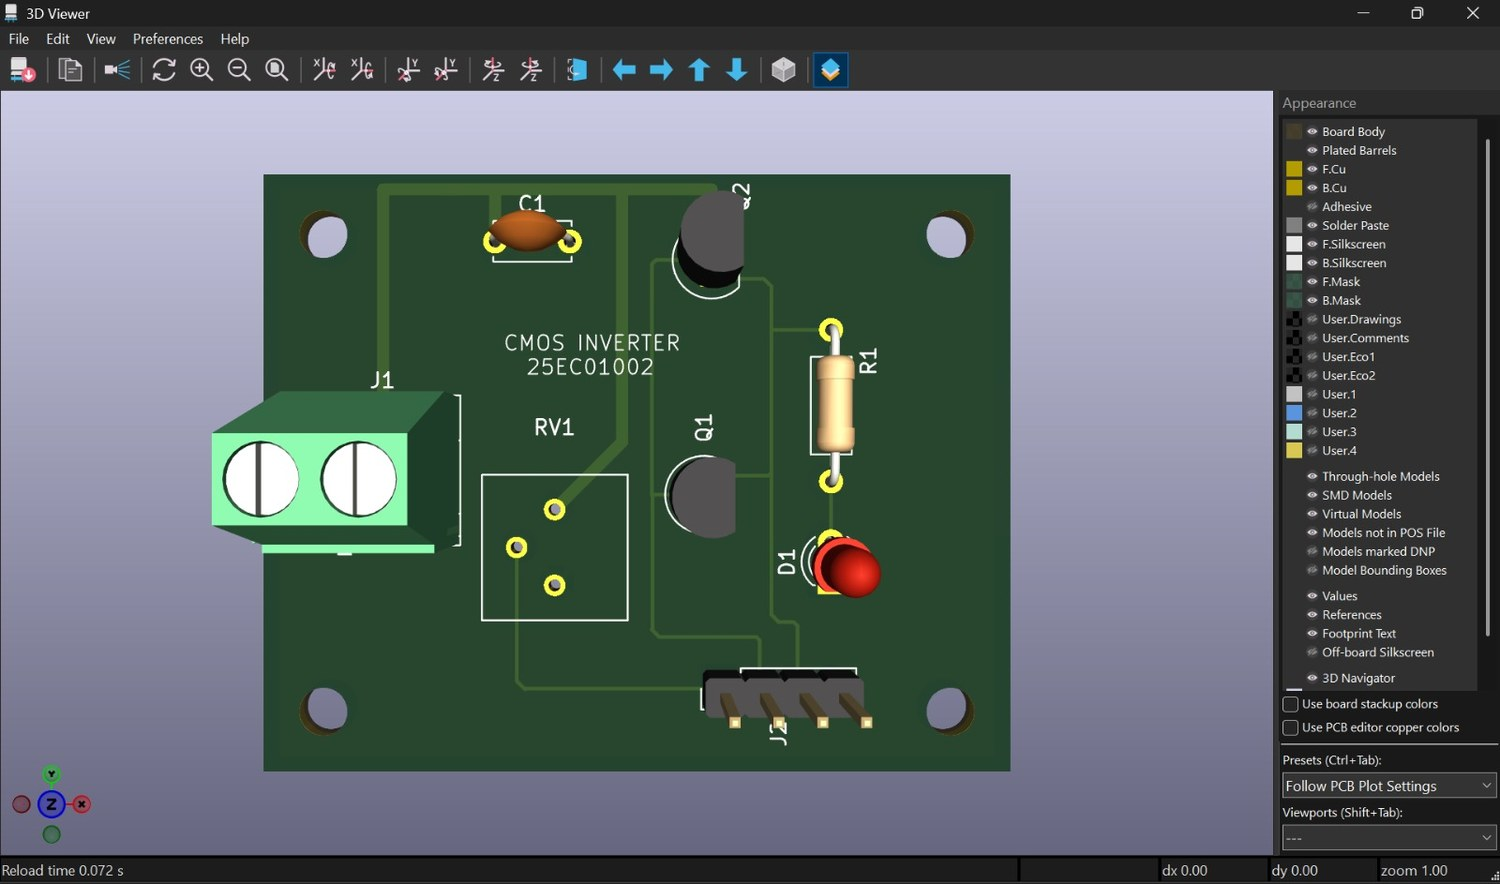
\includegraphics[width=0.84\linewidth]{figures/e3-3d-top.jpg}\caption{3D viewer, top of the board.}\end{figure}
\lab{R}{+5V track resistance, J1 to Q2}
\[R=\frac{\rho L}{w\,t}=\frac{1.68\times10^{-8}\times(47.1\times10^{-3})}{(0.8\times10^{-3})\times(35\times10^{-6})}=0.028\ \Omega\]
\begin{itemize}
\item Measured $L=47.1$ mm, $w=0.8$ mm, $t=35\,\mu$m, $\rho_{Cu}=1.68\times10^{-8}\ \Omega$\,m.
\item Drop at $I=5$ mA (LED 4.25 mA + trimpot 0.5 mA): $\Delta V=0.14$ mV, i.e.\ 0.003 \% of 5 V.
\end{itemize}
\begin{answer}
\begin{itemize}
\item No: even at 0.25 mm, $R\approx0.09\ \Omega$ and $\Delta V\approx0.45$ mV, negligible against the 2.35 V threshold.
\item The 0.8 mm width is for mechanical robustness, not electrical need.
\end{itemize}
\end{answer}

%------------------------------------------------------------ EX 4
\exhead{Exercise 4}{Manufacturing outputs}
\begin{itemize}
\item \ok\ Gerbers plotted to \texttt{gerbers/} \quad \ok\ PTH and NPTH drill files \quad \ok\ BOM exported as CSV
\item \ok\ \texttt{25EC01002\_INV\_gerbers.zip} \quad \ok\ project archive zip
\item Checked in GerbView: outline, drill holes and silkscreen verified.
\item Layers loaded: \textbf{13} (9 Gerber + 2 drill + 2 drill maps); board size read back: \textbf{50.1 $\times$ 40.1 mm} (50 $\times$ 40 mm plus 0.1 mm outline width).
\end{itemize}
\begin{figure}[H]\centering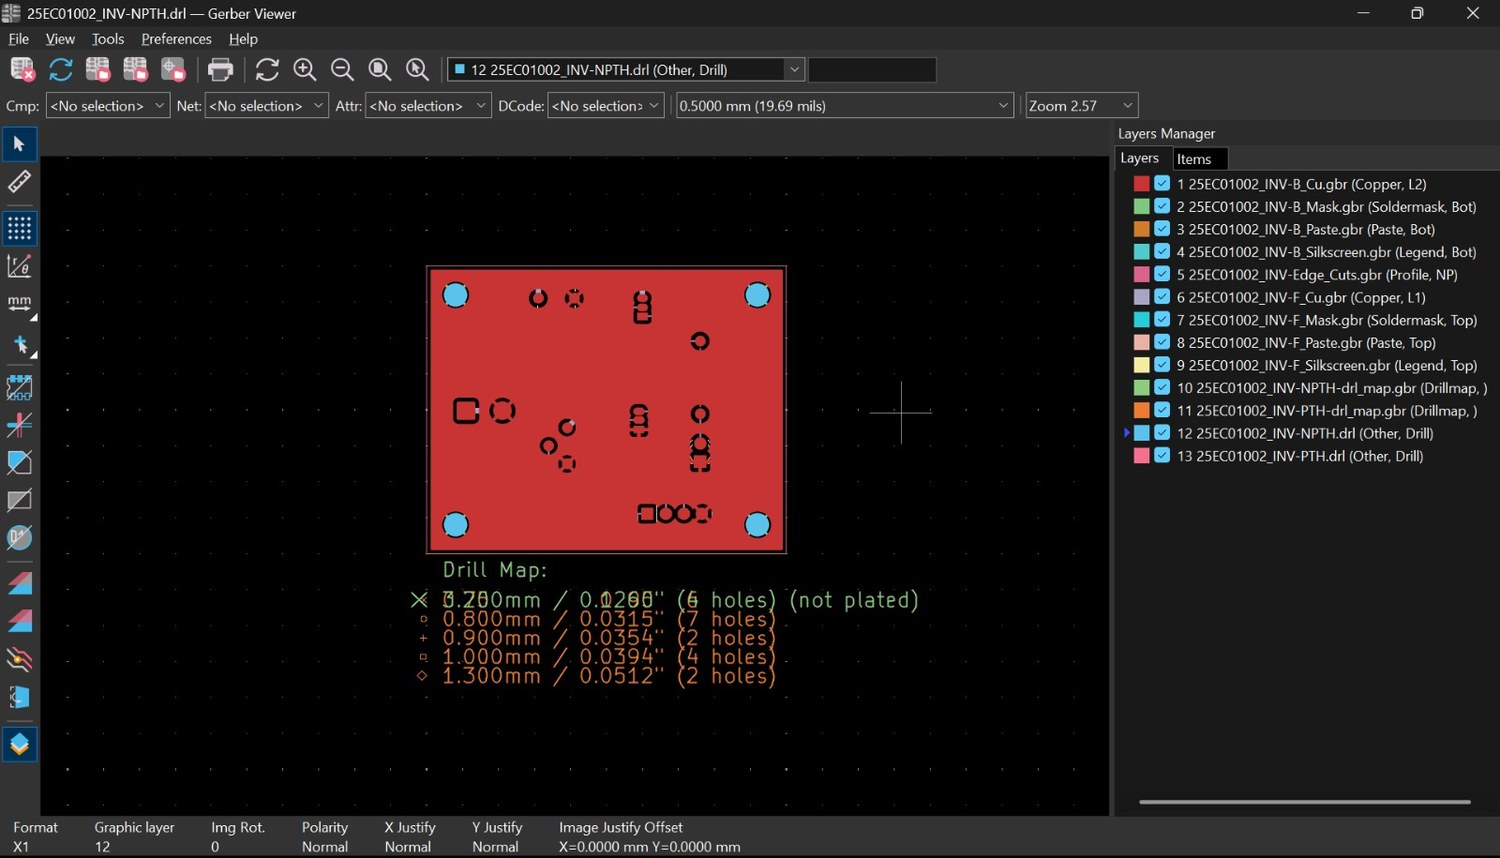
\includegraphics[width=0.84\linewidth]{figures/e4-gerbview.jpg}\caption{GerbView with all layers loaded.}\end{figure}
\begin{answer}
\begin{itemize}
\item File: the plated drill file \texttt{25EC01002\_INV-PTH.drl}.
\item Gerbers hold only the copper rings, no holes; the factory can still quote from size and layer count but would build a board with no lead holes, which is unusable.
\end{itemize}
\end{answer}

%------------------------------------------------------------ EX 5
\exhead{Exercise 5}{Extra explorations: options 1, 2, 3 and 4}
\begin{itemize}
\item All four options were done, each as a single change on its own copy of the Exercise 4 project and never stacked on another, so Exercise 4 is untouched.
\item Folders: \texttt{25EC01002\_INV\_ex5\_opt1} to \texttt{..\_ex5\_opt4}.
\item \textbf{Option 1:} second identical inverter stage, so the board becomes a non-inverting buffer. \textbf{Option 2:} LED lights when the output is low. \textbf{Option 3:} minimum clearance raised to 0.4 mm. \textbf{Option 4:} trimpot replaced by a header, board shrunk.
\end{itemize}

\lab{Option 1}{Non-inverting buffer: a second identical inverter stage}
\begin{itemize}
\item Change: Q3 (2N7000) and Q4 (BS250) added as a copy of the inverter. Stage 1 (Q1, Q2) now drives a new net \texttt{/VOUT1}, which is the gate line of stage 2; R1 and D1 hang on the final output \texttt{/VOUT}. J1, C1, RV1 and J2 are unchanged.
\item Pin labels used below: A = Q2 drain, B = Q1 drain, C = J1 pin 1, D = Q2 source, E = Q4 source, F = Q4 drain, G = R1 pin 1, H = Q3 drain, I = Q4 gate, J = Q3 gate.
\end{itemize}

\lab{1.1}{LTspice: simulate the buffer first}
\begin{itemize}
\item Same models as before, \texttt{2N7000.onsemi.lib} and \texttt{BS250.philips.lib}. Netlists: \texttt{buffer\_DC.cir} and \texttt{buffer\_TRAN.cir}.
\item DC: \texttt{.dc Vin 0 5 0.01}. Transient: \texttt{PULSE(0 5 0 1n 1n 0.5m 1m 3)}, with 1 ns edges so the delays are not hidden by a slow input ramp.
\item The LED here uses the \texttt{LED} model line ($V_F=1.68$ V at 3.3 mA), so its current is not comparable with the 4.25 mA of Exercise 0, where D1 was the default 0.69 V diode.
\end{itemize}
{\footnotesize\ttfamily\raggedright\setlength{\parskip}{1pt}
XN1 out1 in 0 2N7000 \quad XP1 out1 in vdd BS250\par
XN2 out2 out1 0 2N7000 \quad XP2 out2 out1 vdd BS250\par
R1 out2 n002 1k \quad D1 n002 0 LED\par}
\begin{figure}[H]\centering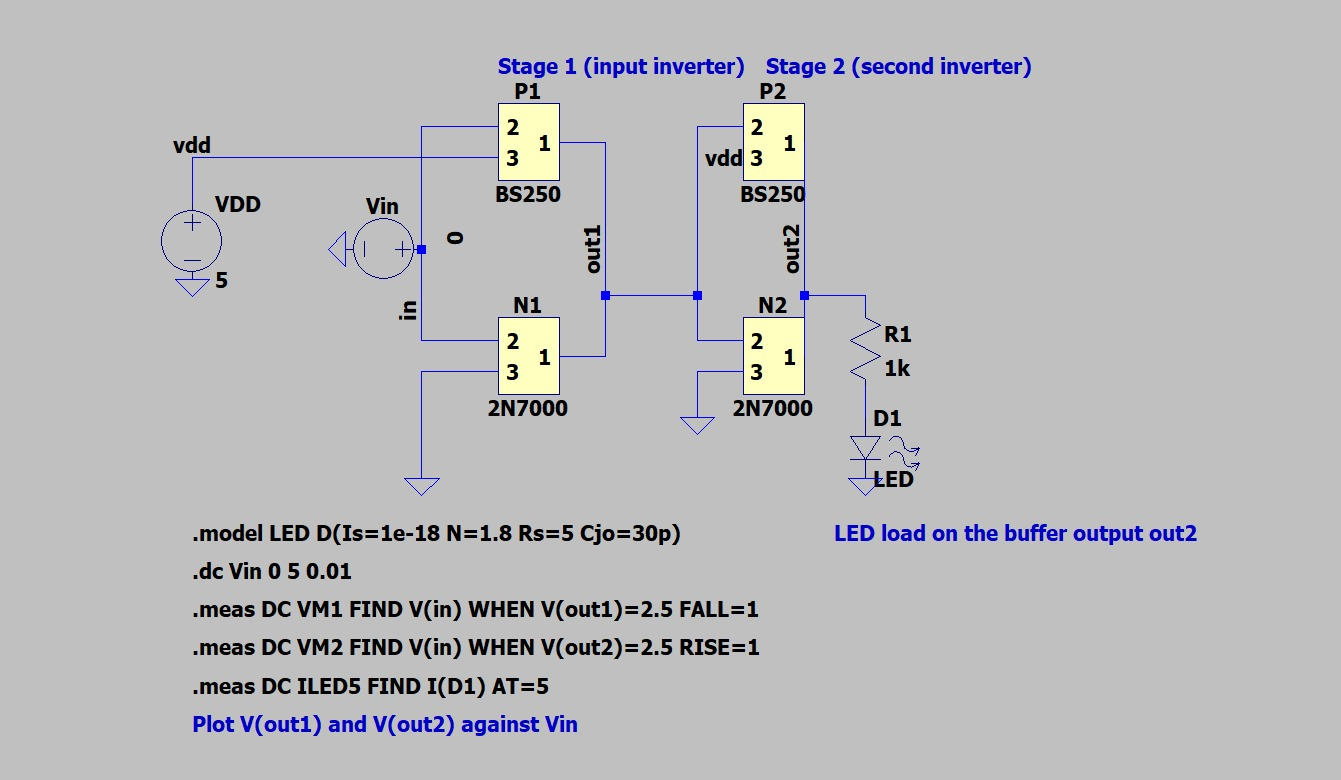
\includegraphics[width=0.8\linewidth]{figures/e5o1-dc-circuit.jpg}\caption{LTspice circuit for the DC sweep: stage 1 (P1, N1) drives stage 2 (P2, N2) through \texttt{out1}; R1 and D1 load the buffer output \texttt{out2}.}\end{figure}
\begin{figure}[H]\centering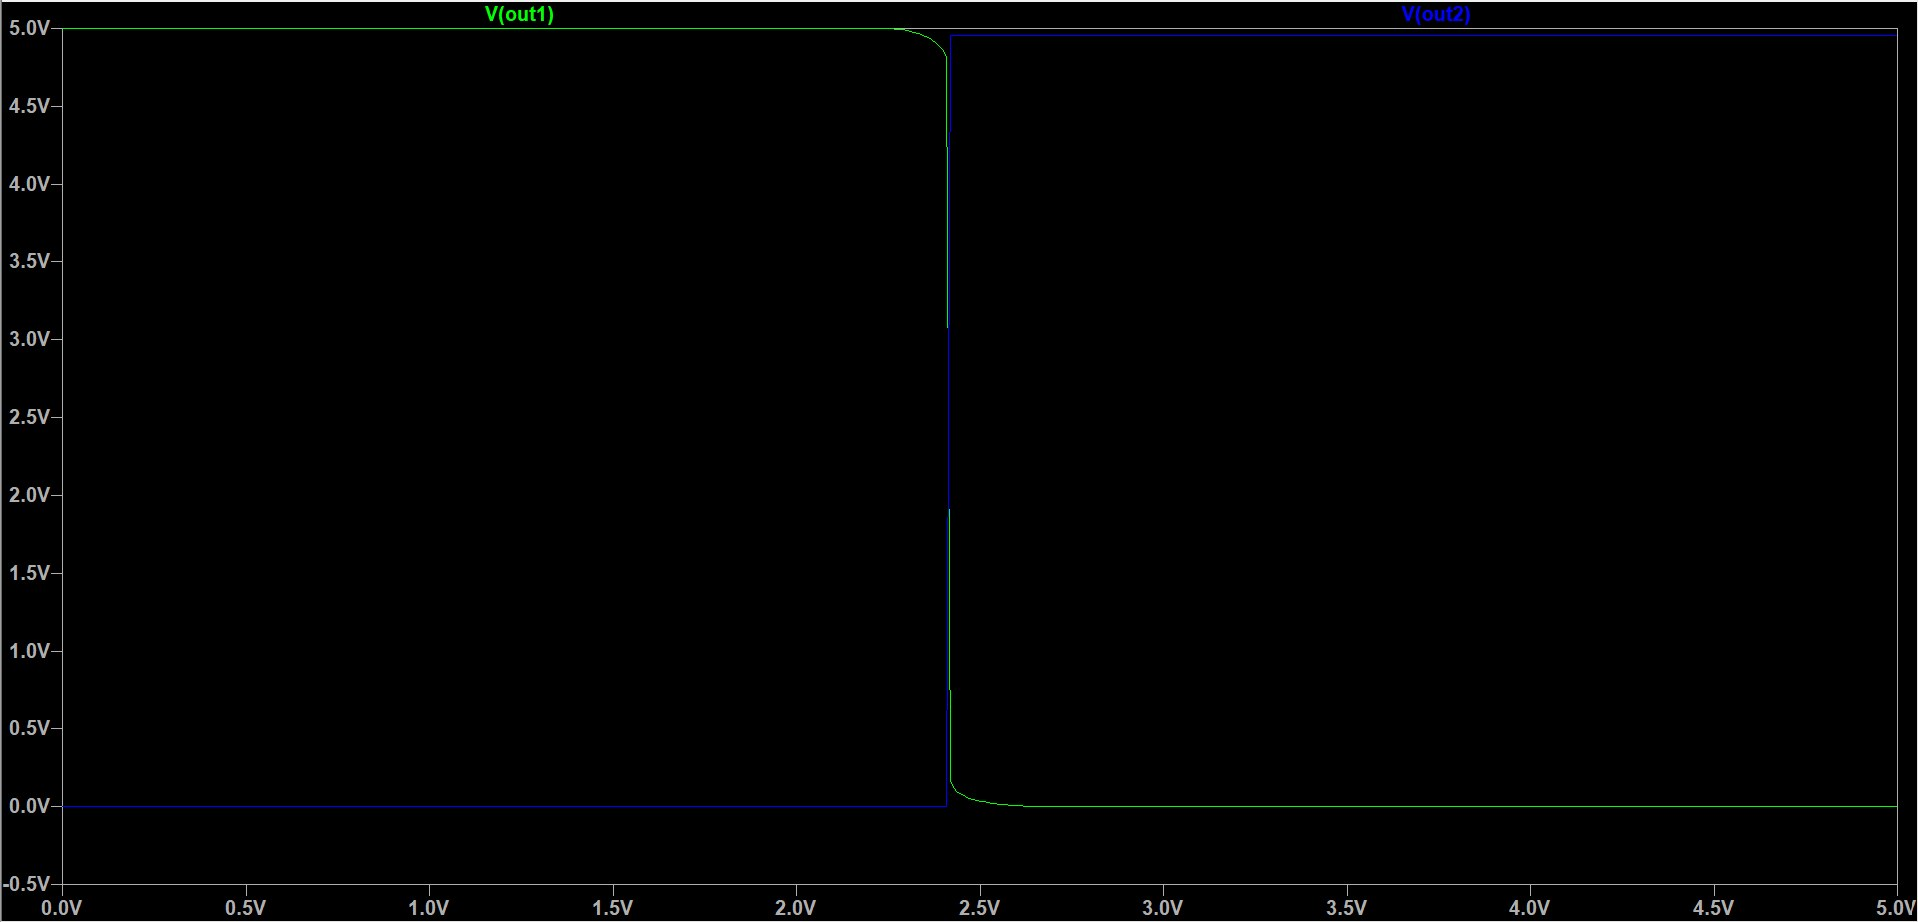
\includegraphics[width=0.8\linewidth]{figures/e5o1-dc.jpg}\caption{\texttt{.dc Vin 0 5 0.01}: V(out1) falls and V(out2) rises at the same $V_{IN}$.}\end{figure}
\begin{figure}[H]\centering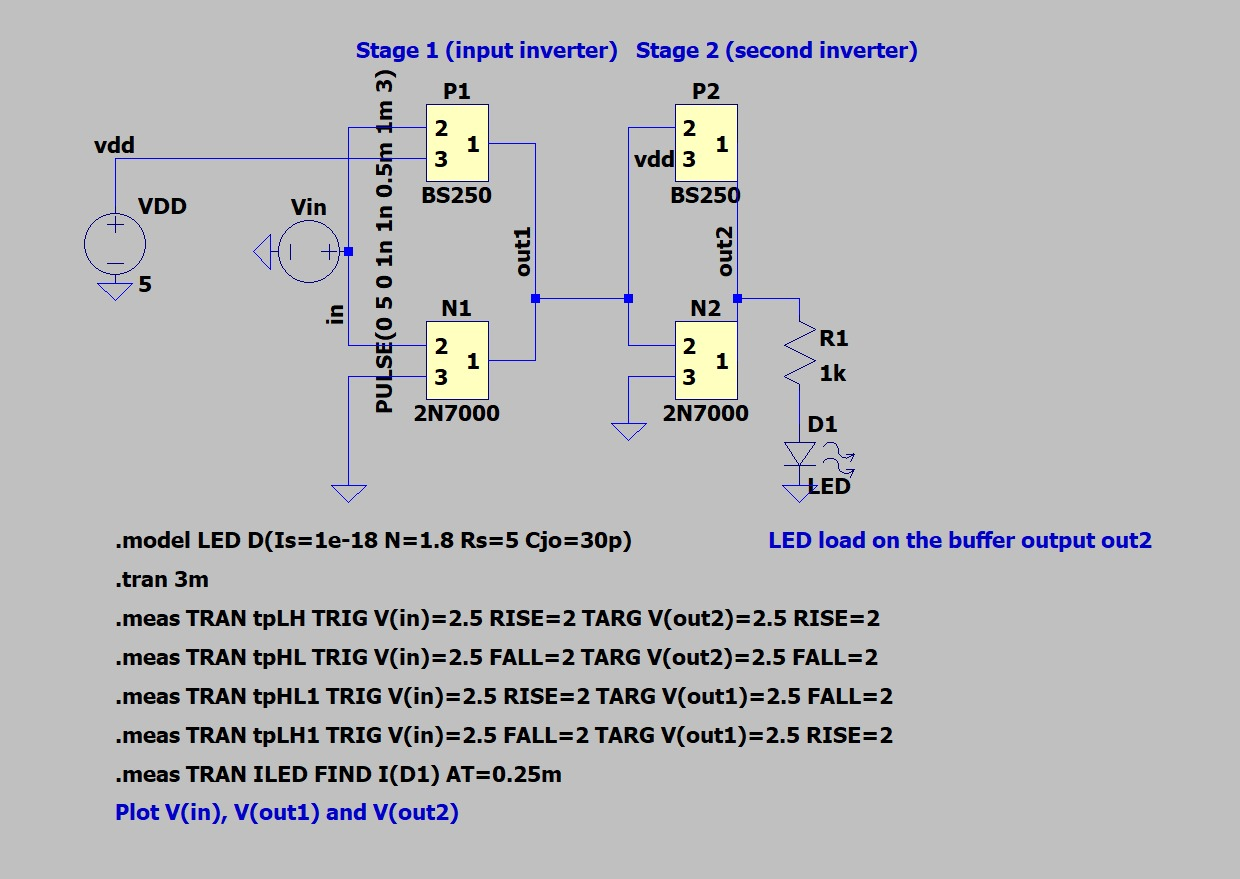
\includegraphics[width=0.8\linewidth]{figures/e5o1-tran-circuit.jpg}\caption{LTspice circuit for the transient run: the same buffer with a 0--5 V, 1 kHz pulse source and the delay \texttt{.meas} lines.}\end{figure}
\begin{figure}[H]\centering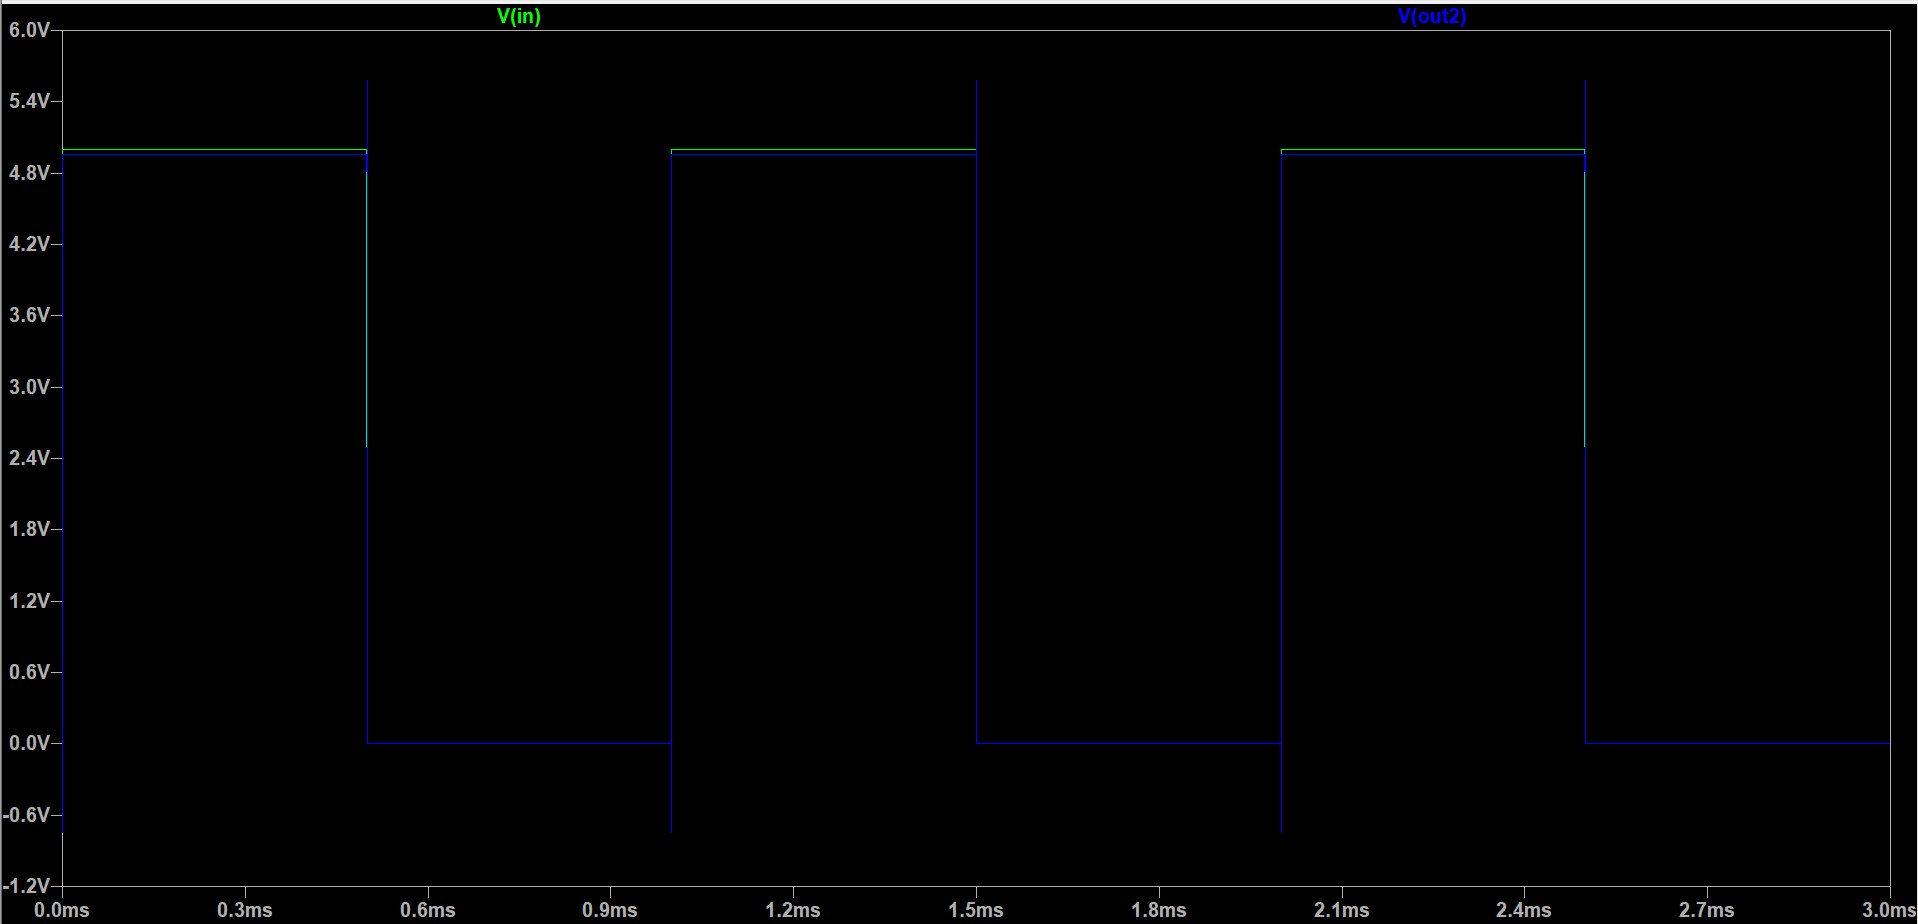
\includegraphics[width=0.8\linewidth]{figures/e5o1-tran.jpg}\caption{\texttt{.tran 3m}: V(out2) follows V(in), same polarity.}\end{figure}
\begin{figure}[H]\centering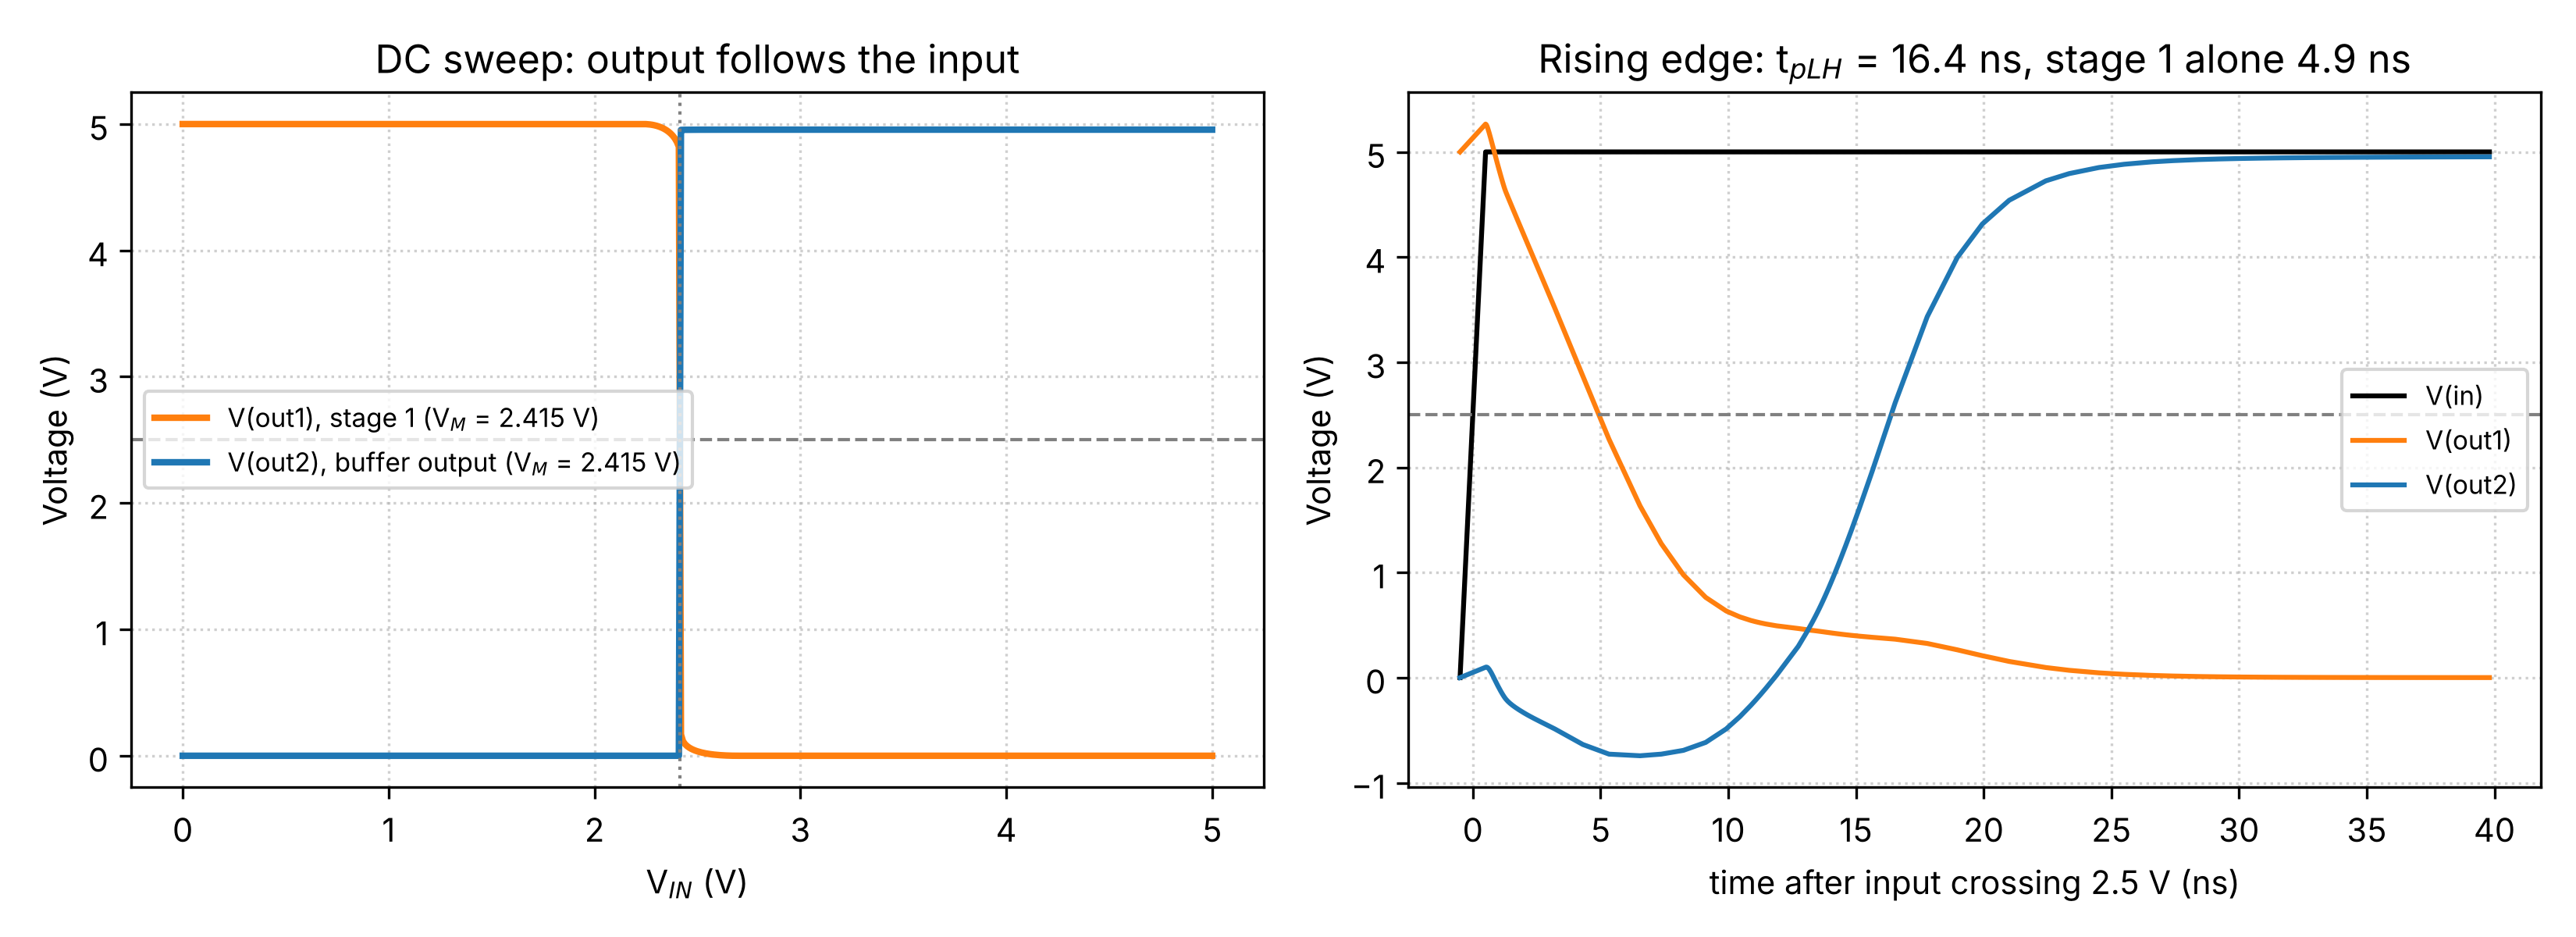
\includegraphics[width=\linewidth]{figures/e5o1-buffer.png}\caption{Left: VTC of stage 1 and of the buffer. Right: rising-edge delay of the buffer against stage 1 alone (from the LTspice raw file).}\end{figure}
\begin{table}[H]\centering\small\sffamily
\begin{tabular}{@{}lcc@{}}\rowcolor{teal}\color{white}\textbf{Quantity}&\color{white}\textbf{Stage 1 (out1)}&\color{white}\textbf{Buffer (out2)}\\
$V_M$ ($V_{OUT}=2.5$ V)&2.415 V (falling)&2.415 V (rising)\\
\rowcolor{mist}$V_{OH}$ / $V_{OL}$&5.00 V / $\approx0$ V&4.956 V / $\approx0$ V\\
Delay, input rising&4.9 ns&$t_{pLH}$ = 16.4 ns\\
\rowcolor{mist}Delay, input falling&7.8 ns&$t_{pHL}$ = 16.8 ns\\
$I_{LED}$&--&0 at $V_{IN}=0$; 3.28 mA at $V_{IN}=5$ V\\\end{tabular}
\caption{Simulation results, from the \texttt{.meas} lines and the DC export.}\end{table}
\begin{itemize}
\item Hand check: $(V_{OH}-V_F)/R_1=(4.956-1.68)/1\,\mathrm{k}\Omega=3.28$ mA against 3.276 mA simulated.
\item $V_M$ is 2.415 V here against 2.349 V for the single inverter, because stage 1 now drives only gates and no longer has the R1/LED load on its output.
\item At the input edges V(out2) briefly dips to $-0.74$ V and overshoots to 5.58 V for a few ns, probably gate--drain capacitance feeding the 1 ns edge to the output; not investigated further.
\end{itemize}
\begin{answer}
\textbf{Why is it non-inverting?}
\begin{itemize}
\item Stage 1 inverts $V_{IN}$ into $V_{OUT1}$ and stage 2 inverts $V_{OUT1}$ again, so $V_{OUT}$ has the same polarity as $V_{IN}$.
\item Simulated: V(out2) is low below 2.415 V and high above it, so the LED now lights when $V_{IN}$ is high (it lit when $V_{IN}$ was low in Exercise 4).
\item Stage 1 swings almost rail to rail, so stage 2 always sees a clean logic level and the threshold stays at $V_M$ of stage 1.
\item The price is delay: 16.4 ns for the buffer, of which 4.9 ns is stage 1 and about 11.5 ns is stage 2, which also drives the LED branch.
\end{itemize}
\end{answer}

\lab{1.2}{KiCad: schematic, board and manufacturing files}
\begin{itemize}
\item Schematic: Q3 and Q4 copied from Q1 and Q2 (Q4 flipped so its source faces +5V); net \texttt{/VOUT1} joins A, B, I and J; R1, D1 and J2 pin 3 are on \texttt{/VOUT}. ERC \textbf{0 errors, 0 warnings}; netlist update (F8) \textbf{0 warnings, 0 errors}.
\item Board: Q3 and Q4 use \texttt{TO-92\_Inline} like Q1 and Q2. The 50 $\times$ 40 mm outline and the four M3 holes did not change.
\item Routed on F.Cu with 0.25 mm signal and 0.8 mm +5V tracks, no vias, GND from the B.Cu pour. DRC \textbf{0 violations, 0 unconnected items, 0 schematic-parity errors} (31 pads, 7 nets, 52 track segments).
\item Gerbers and both drill files re-plotted to \texttt{gerbers\_ex5\_opt1/} and loaded back into GerbView (13 entries): 27 plated holes (21 + 6 new) and 4 non-plated.
\end{itemize}
\begin{figure}[H]\centering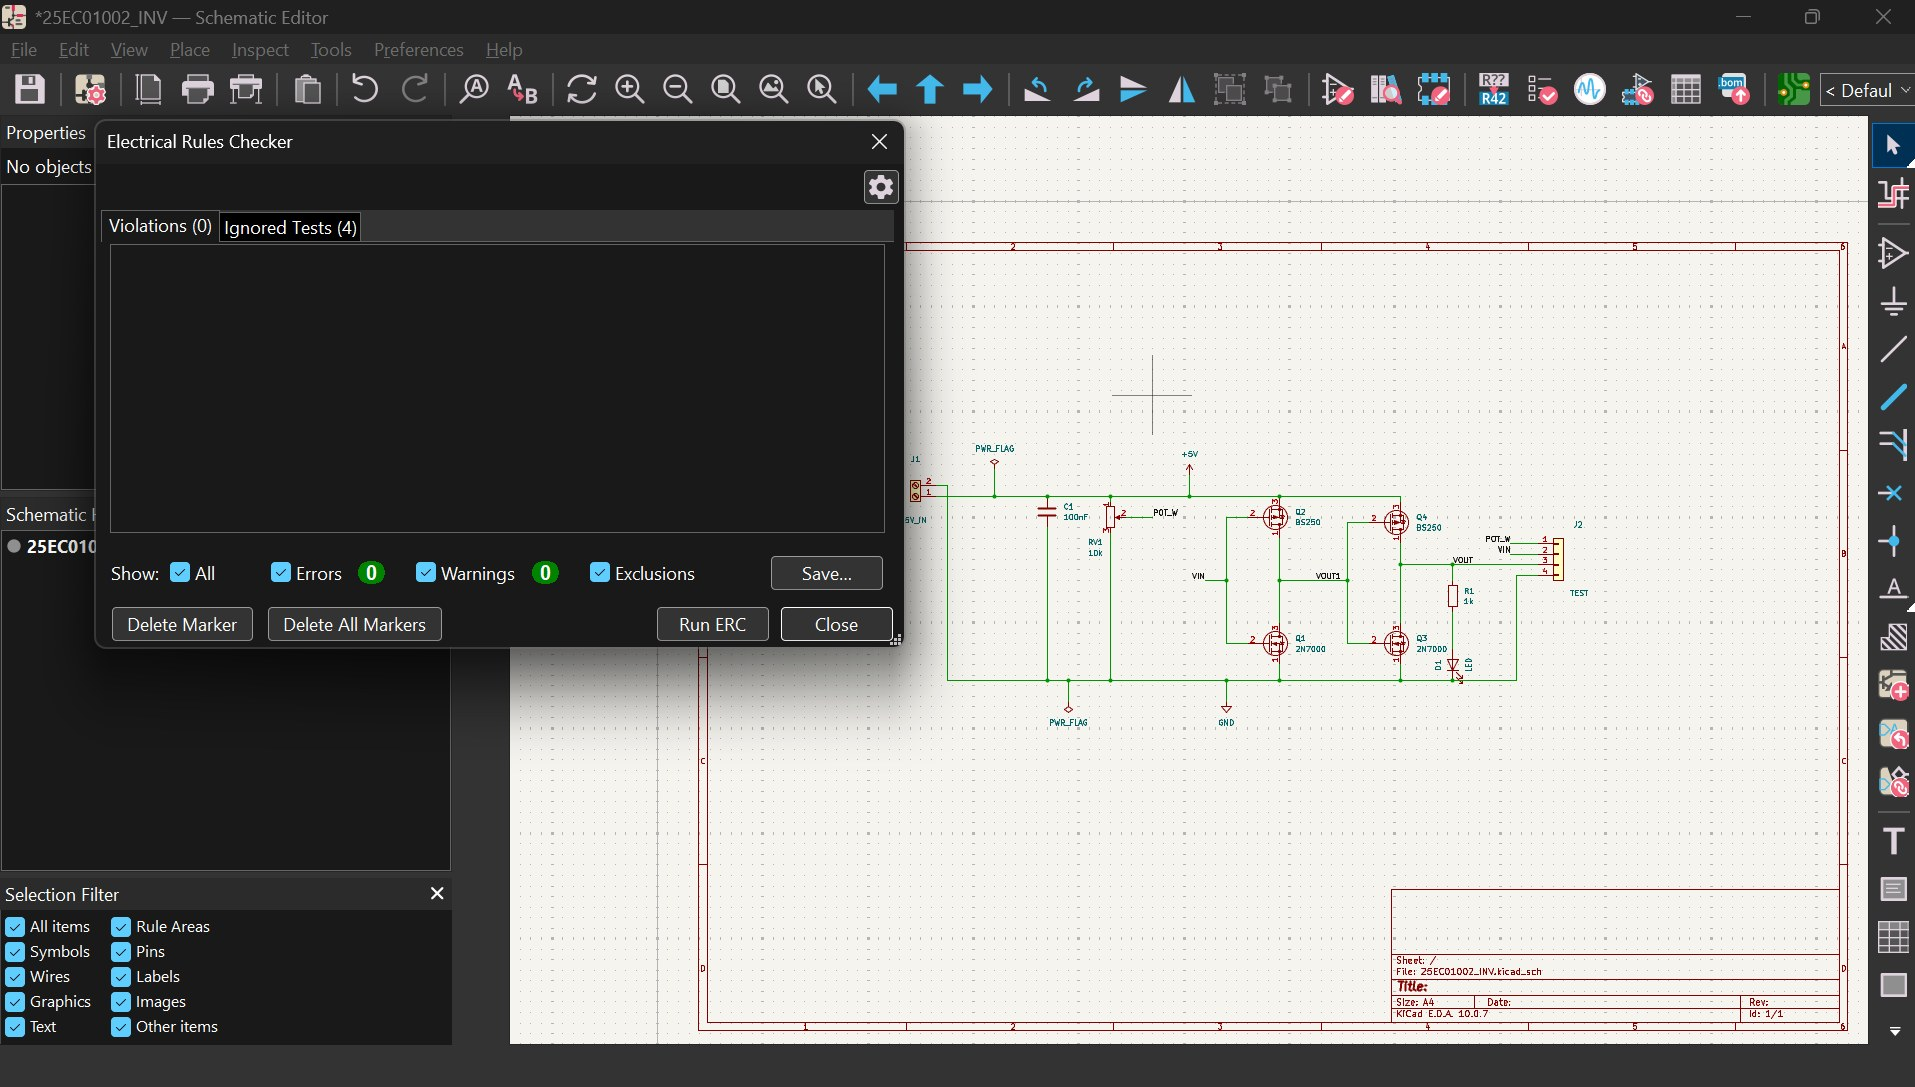
\includegraphics[width=0.84\linewidth]{figures/e5o1-erc.jpg}\caption{Option 1 schematic: ERC 0 errors, 0 warnings.}\end{figure}
\begin{figure}[H]\centering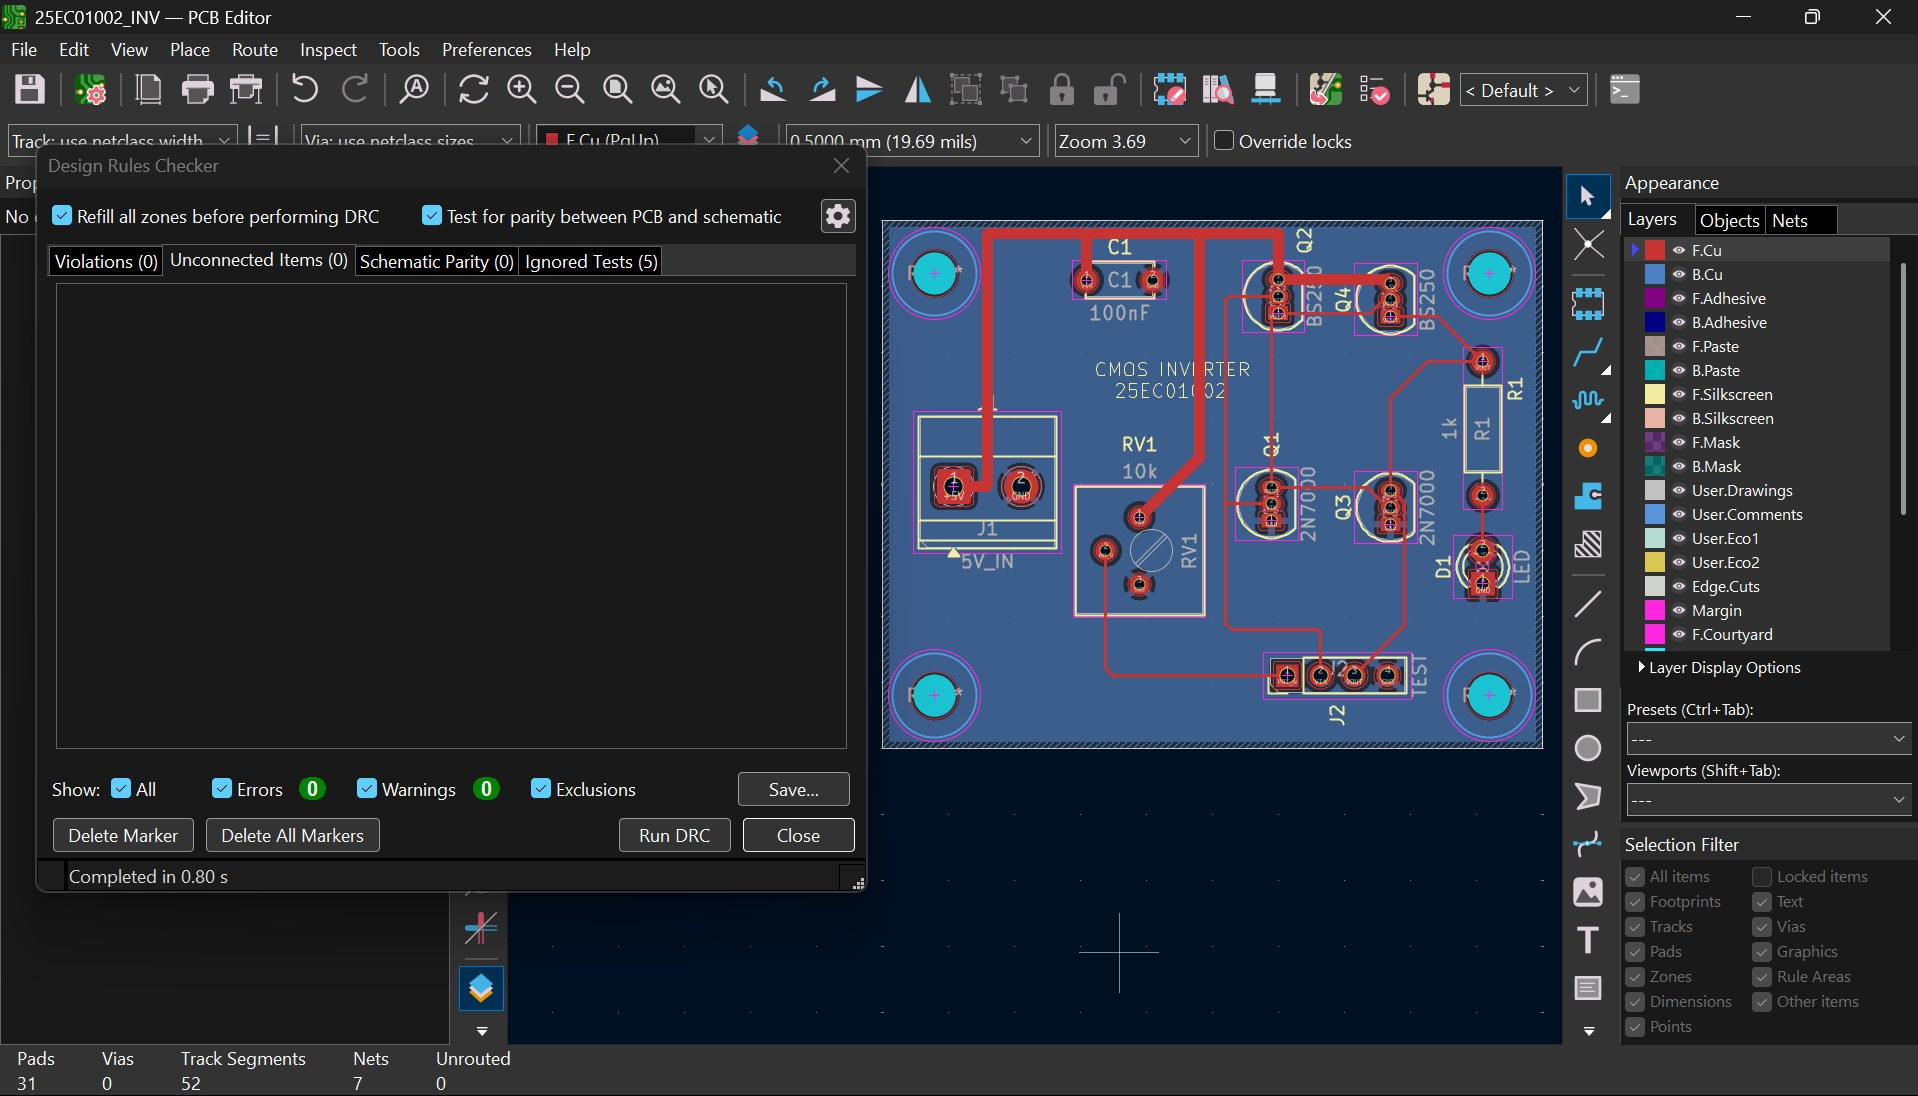
\includegraphics[width=0.84\linewidth]{figures/e5o1-drc.jpg}\caption{Option 1 board: DRC with Violations, Unconnected Items and Schematic Parity all 0.}\end{figure}
\begin{figure}[H]\centering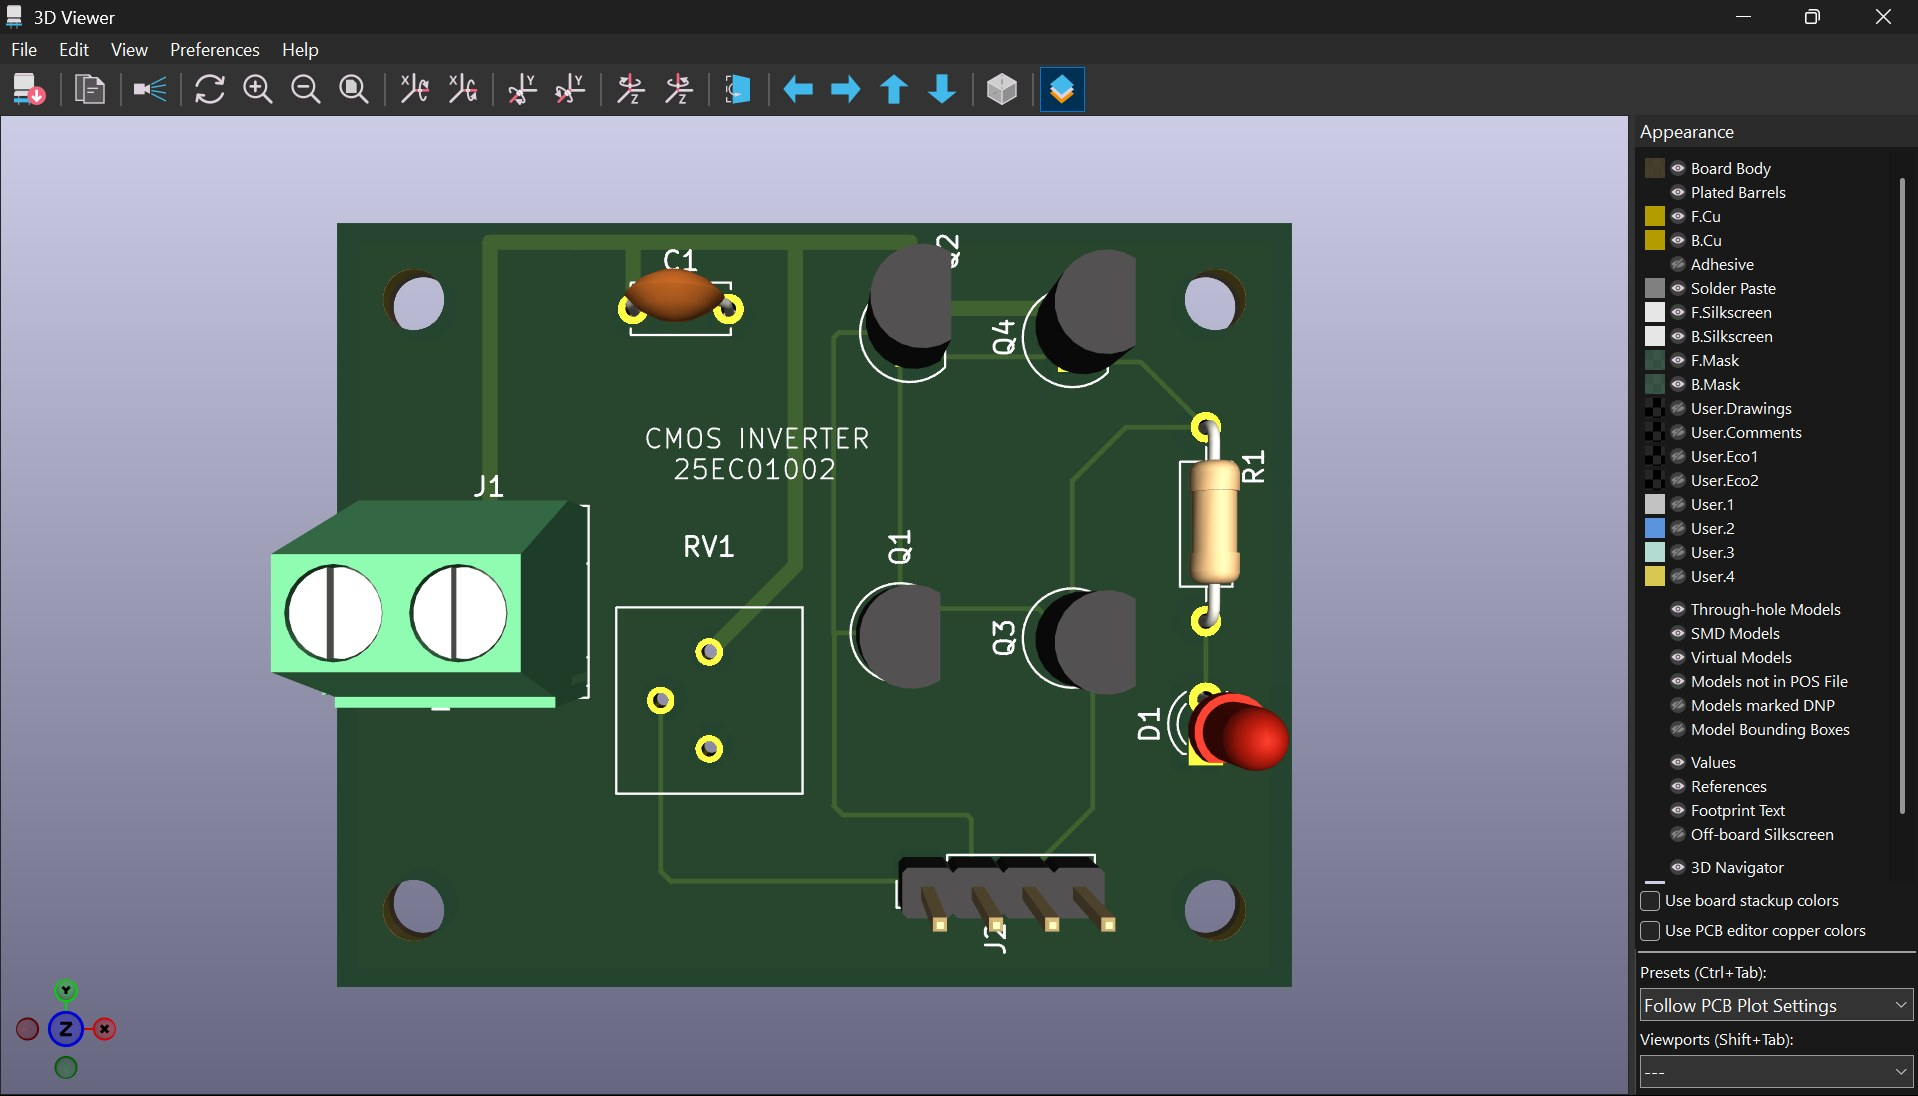
\includegraphics[width=0.84\linewidth]{figures/e5o1-3d.jpg}\caption{Option 1 board in the 3D viewer, top side.}\end{figure}
\begin{figure}[H]\centering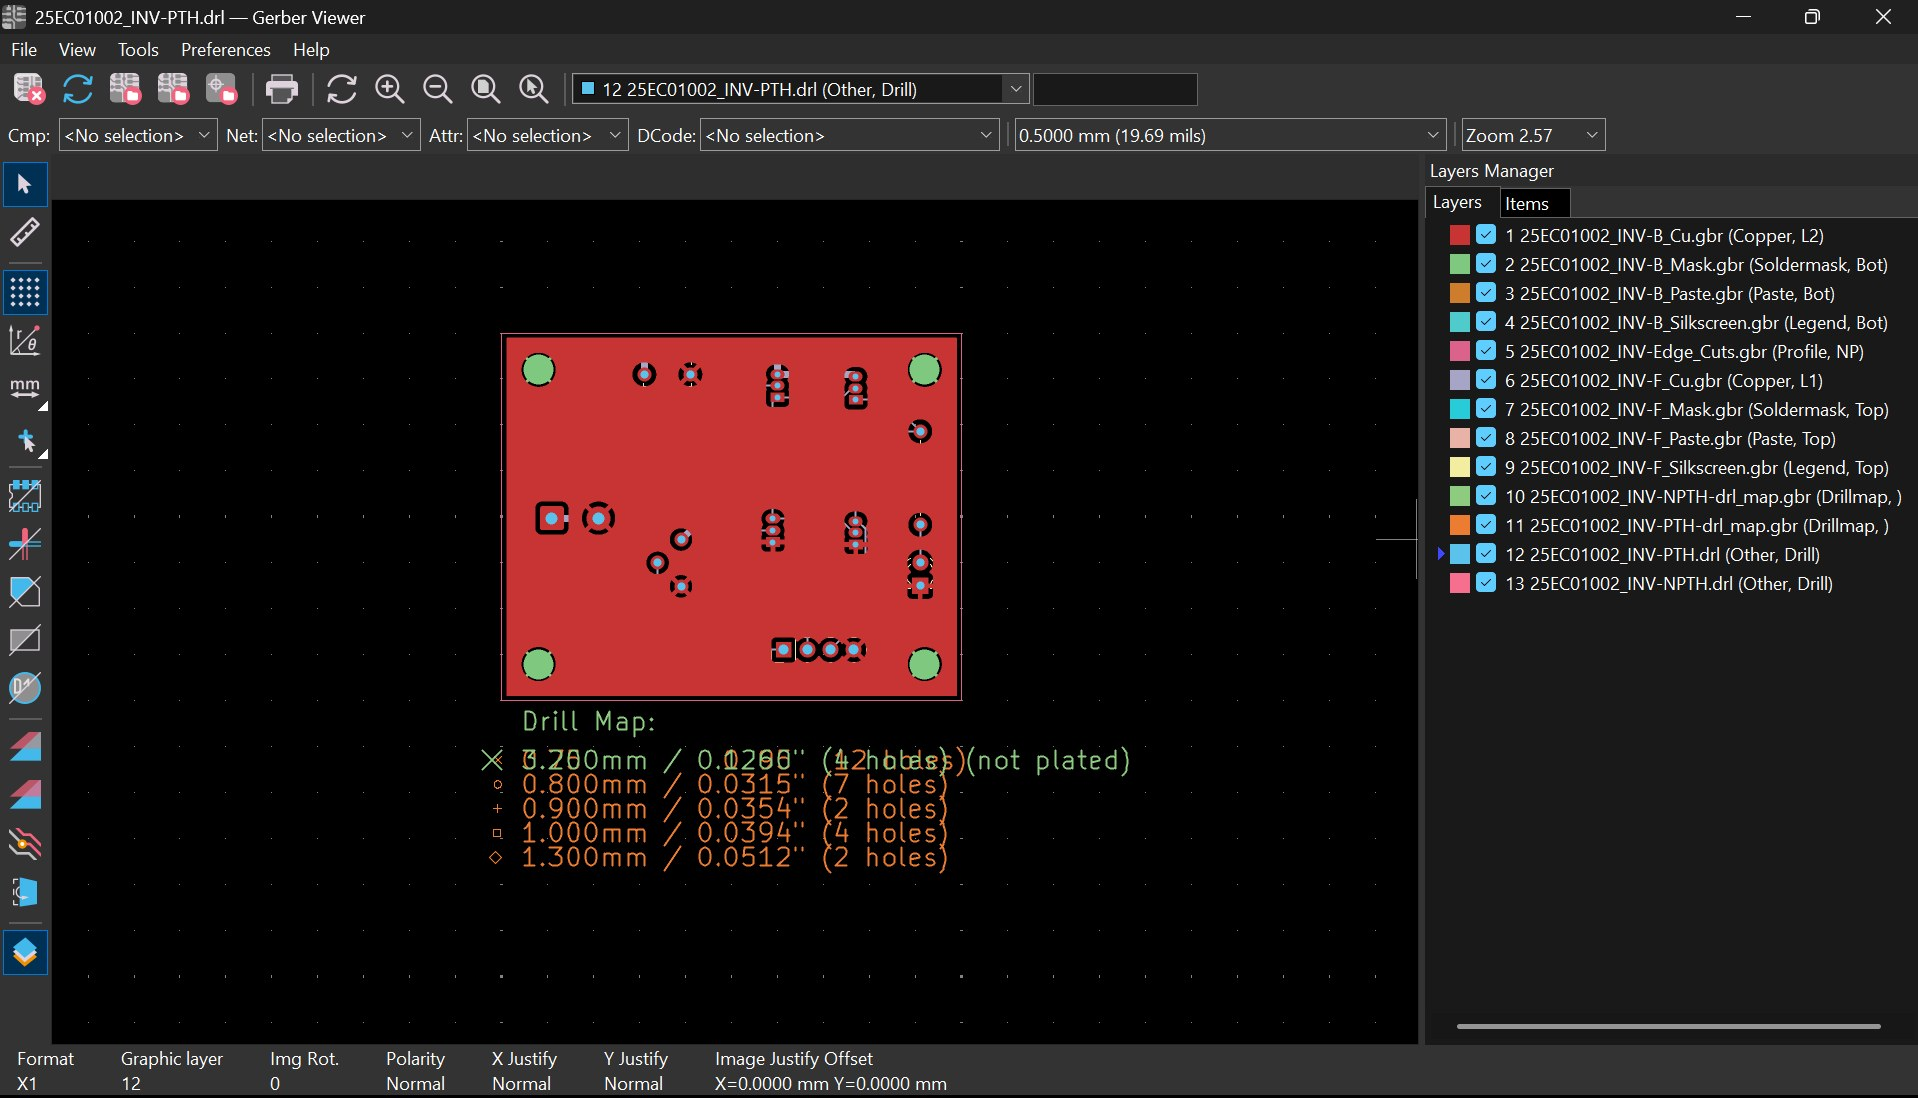
\includegraphics[width=0.84\linewidth]{figures/e5o1-gerbview.jpg}\caption{GerbView with the option 1 Gerbers and drill files loaded.}\end{figure}

\Needspace{20\baselineskip}
\lab{1.3}{Does the placement still work, and what did it cost?}
\begin{table}[H]\centering\small\sffamily
\begin{tabular}{@{}lcc@{}}\rowcolor{teal}\color{white}\textbf{Item}&\color{white}\textbf{Exercise 4}&\color{white}\textbf{Option 1}\\
Board size&50 $\times$ 40 mm&50 $\times$ 40 mm\\
\rowcolor{mist}Pads / nets&25 / 6&31 / 7\\
Footprints moved&--&R1, D1: 7.5 mm to the right\\
\rowcolor{mist}Footprints added&--&Q3, Q4\\
+5V copper&102.9 mm&111.5 mm\\
\rowcolor{mist}VIN copper&42.9 mm&42.9 mm\\
VOUT copper&41.65 mm&40.23 mm\\
\rowcolor{mist}VOUT1 copper (new net)&--&32.21 mm\\
All tracks&214.5 mm (44 segments)&253.9 mm (52 segments)\\
\rowcolor{mist}Vias&0&0\\
Q2 drain (A) to Q1 drain (B), straight line&13.20 mm&13.20 mm\\
\rowcolor{mist}J1 pin 1 (C) to Q2 source (D), straight line&29.12 mm&29.12 mm\\
J1 pin 1 (C) to Q4 source (E), straight line&--&36.47 mm\\
\rowcolor{mist}Output drain to R1 pin 1 (G): A--G / F--G&8.71 mm&7.79 mm\\
Q4 drain (F) to Q3 drain (H), straight line&--&13.19 mm\\
\rowcolor{mist}Q2 drain (A) to Q4 gate (I)&--&8.57 mm\\
Q1 drain (B) to Q3 gate (J)&--&9.15 mm\\
\rowcolor{mist}+5V path, J1 to Q2 (routed)&47.1 mm (0.028 $\Omega$)&47.1 mm (0.028 $\Omega$)\\
+5V path, J1 to Q4 (routed)&--&55.7 mm (0.034 $\Omega$)\\\end{tabular}
\caption{Layout cost of option 1, measured from the two \texttt{.kicad\_pcb} files.}\end{table}
\begin{answer}
\textbf{Does the placement still work?}
\begin{itemize}
\item Yes. The ratsnest is not harder to untangle because stage 2 is a copy of stage 1 placed beside it, and the original parts (Q1, Q2, C1, RV1, J1, J2) did not move.
\item The only moves: R1 and D1 shifted 7.5 mm right to free a column at x = 138.5 mm for Q3 and Q4. The outline and the mounting holes are unchanged.
\item It is tight: R1 and D1 are now 4.5 mm from the board edge, so a third stage would need a larger board.
\end{itemize}
\textbf{What it cost:}
\begin{itemize}
\item Board area: none. Copper: +39.4 mm (+18 \%), 8 more segments, 6 more pads, one more net, no vias.
\item Longest new link: C--E, 36.5 mm straight (55.7 mm routed), adding 8.6 mm of +5V copper. Its resistance is 0.034 $\Omega$, about 0.17 mV at 5 mA, negligible; the original J1--Q2 path is unchanged.
\item The new \texttt{/VOUT1} node carries 32.2 mm of 0.25 mm track ($\approx0.06\ \Omega$) and two gate capacitances; at 1 kHz this is negligible, but it is part of the 16 ns delay.
\item The A--B drain link is unchanged at 13.20 mm, and the drain-to-R1 run is 0.9 mm shorter because R1 now sits beside Q4.
\end{itemize}
\end{answer}

\lab{Option 2}{LED lights when the output is low}
\begin{itemize}
\item Change: R1 and D1 were moved from ``VOUT to GND'' to ``+5V to VOUT'', with D1 anode towards R1 and cathode on VOUT. Every other part, value and footprint is unchanged.
\item As in L1, D1 resolves to the default diode, so $V_F=0.69$ V.
\end{itemize}

\lab{2.1}{LTspice: simulate the change first}
\begin{figure}[H]\centering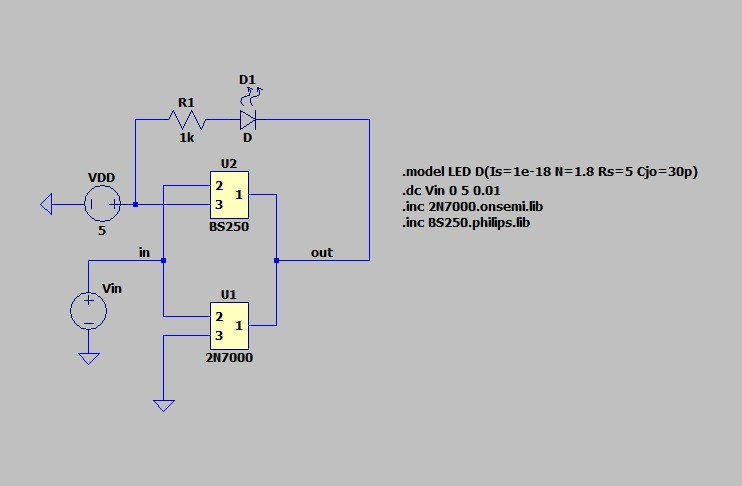
\includegraphics[width=0.62\linewidth]{figures/e5-circuit.jpg}\caption{LTspice circuit with the LED branch from +5 V to \texttt{out}.}\end{figure}
\begin{figure}[H]\centering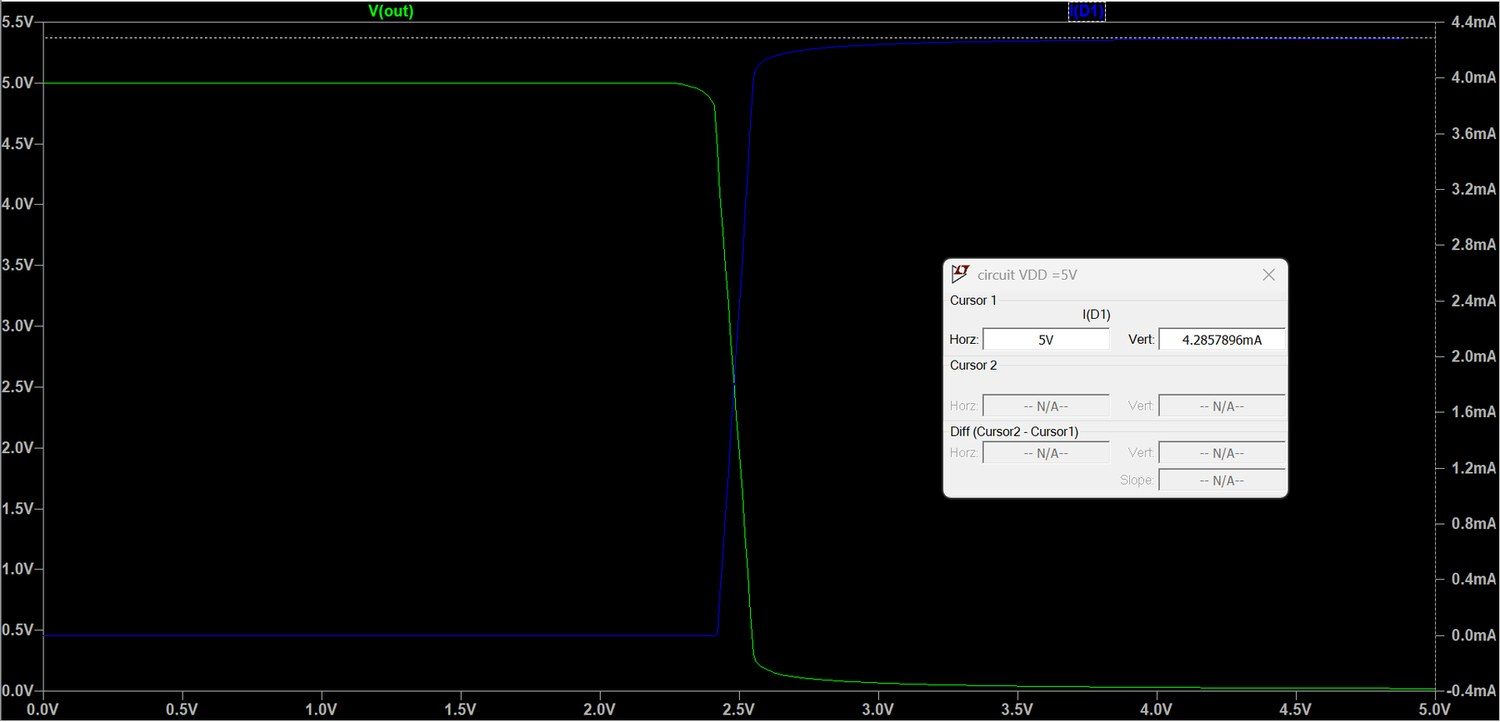
\includegraphics[width=0.9\linewidth]{figures/e5-ltspice-plot.jpg}\caption{\texttt{.dc Vin 0 5 0.01}: V(out) and I(D1); cursor reads 4.286 mA at $V_{IN}=5$ V.}\end{figure}
\begin{figure}[H]\centering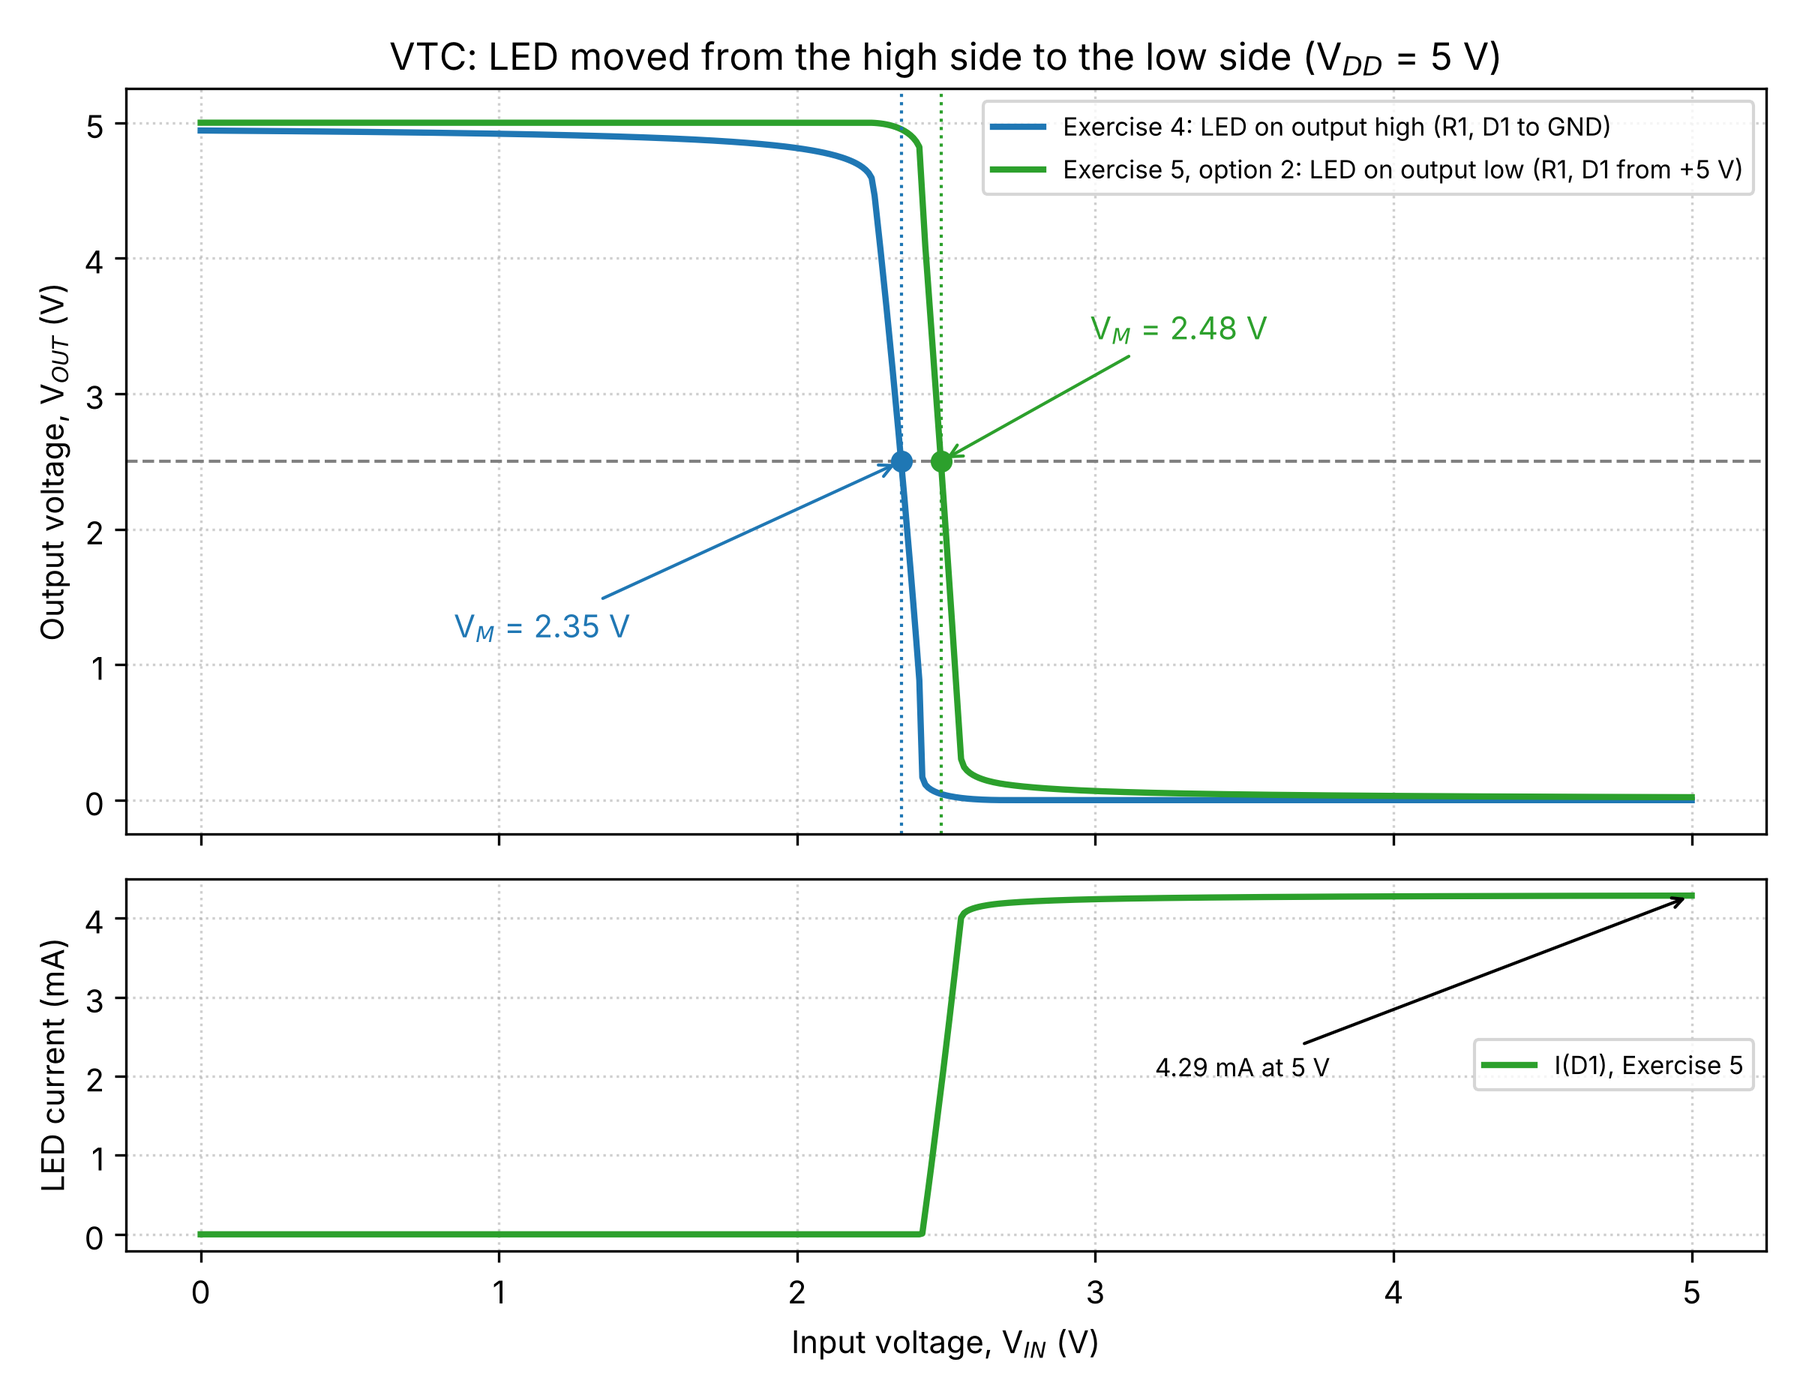
\includegraphics[width=0.78\linewidth]{figures/e5-vtc-compare.png}\caption{VTC of Exercise 4 and Exercise 5 on the same axes, with $V_M$ marked.}\end{figure}
\begin{table}[H]\centering\small\sffamily
\begin{tabular}{@{}lcc@{}}\rowcolor{teal}\color{white}\textbf{Quantity}&\color{white}\textbf{Exercise 4}&\color{white}\textbf{Option 2}\\
$V_M$ ($V_{OUT}=2.5$ V)&2.35 V&2.48 V\\
\rowcolor{mist}$V_{OH}$&4.94 V&5.00 V\\
$V_{OL}$&$\approx0$ V&0.021 V\\
\rowcolor{mist}LED lit when&$V_{IN}$ below about 2.3 V&$V_{IN}$ above about 2.5 V\\
$I_{LED}$&4.25 mA (at $V_{IN}=0$)&4.29 mA (at $V_{IN}=5$ V)\\
\rowcolor{mist}Device carrying $I_{LED}$&BS250 (PMOS)&2N7000 (NMOS)\\\end{tabular}
\caption{Simulation results before and after the change.}\end{table}
\begin{itemize}
\item Hand check: $(V_{DD}-V_F-V_{OL})/R_1=(5-0.69-0.021)/1\,\mathrm{k}\Omega=4.29$ mA against 4.286 mA simulated, within 0.1 \%.
\end{itemize}

\lab{2.2}{KiCad: schematic, board and manufacturing files}
\begin{itemize}
\item Schematic: only two connections changed (D1 pin 1 from GND to \texttt{/VOUT}, R1 pin 1 from \texttt{/VOUT} to +5V). ERC \textbf{0 errors, 0 warnings}; netlist update (F8) \textbf{0 warnings, 0 errors}.
\item Board: re-routed on F.Cu with the same placement and zones refilled. DRC \textbf{0 violations, 0 unconnected items, 0 schematic-parity errors}.
\item Gerbers and both drill files re-plotted to \texttt{gerbers\_ex5/}; the plated and non-plated drill files are identical to Exercise 4 because no hole moved. All layers were loaded back into GerbView.
\end{itemize}
\begin{figure}[H]\centering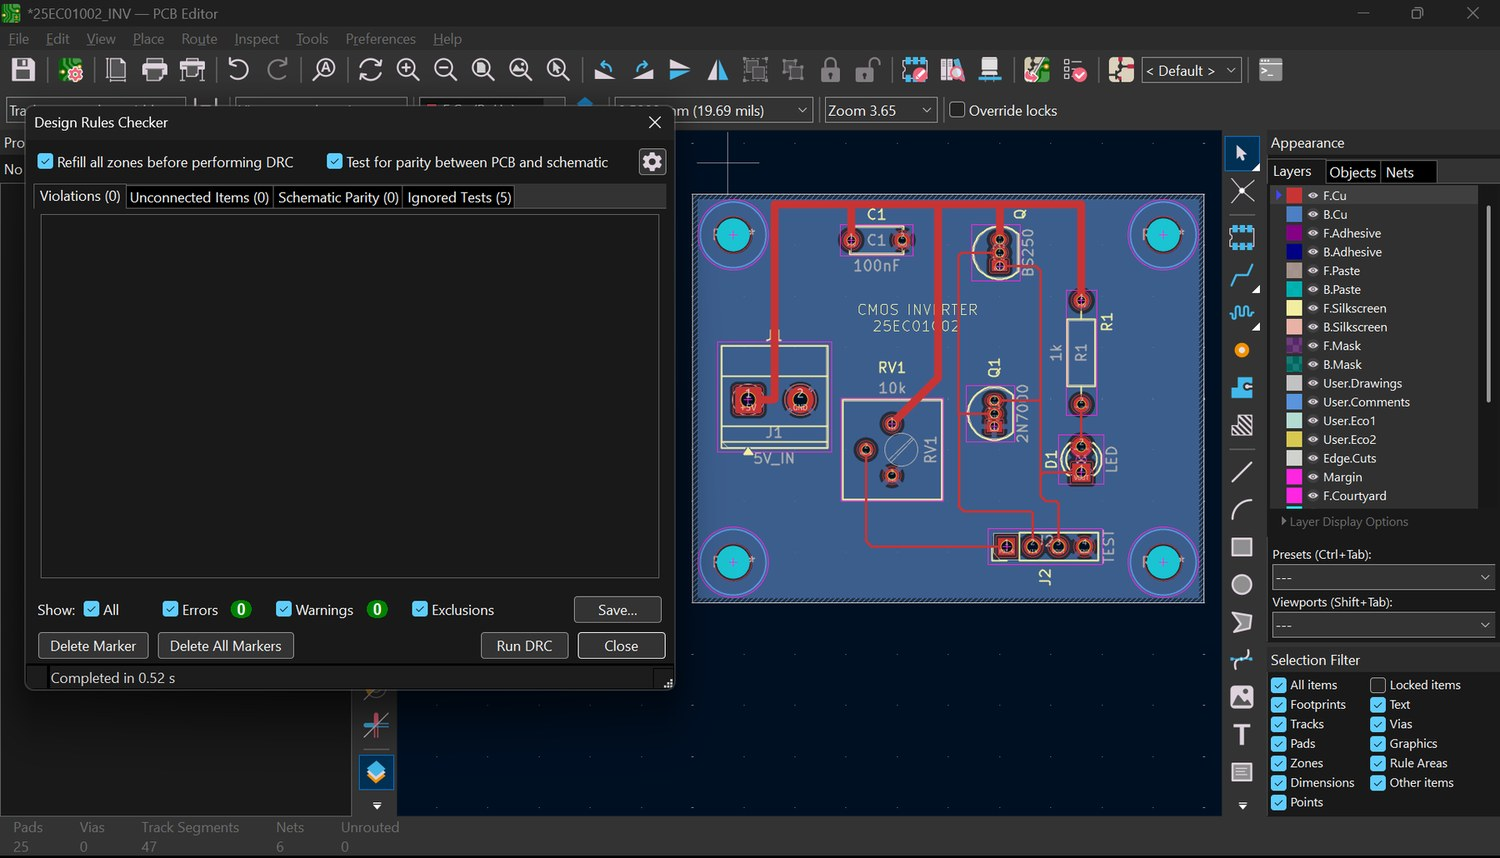
\includegraphics[width=0.84\linewidth]{figures/e5-drc.jpg}\caption{Exercise 5 board: DRC with Violations, Unconnected Items and Schematic Parity all 0.}\end{figure}
\begin{figure}[H]\centering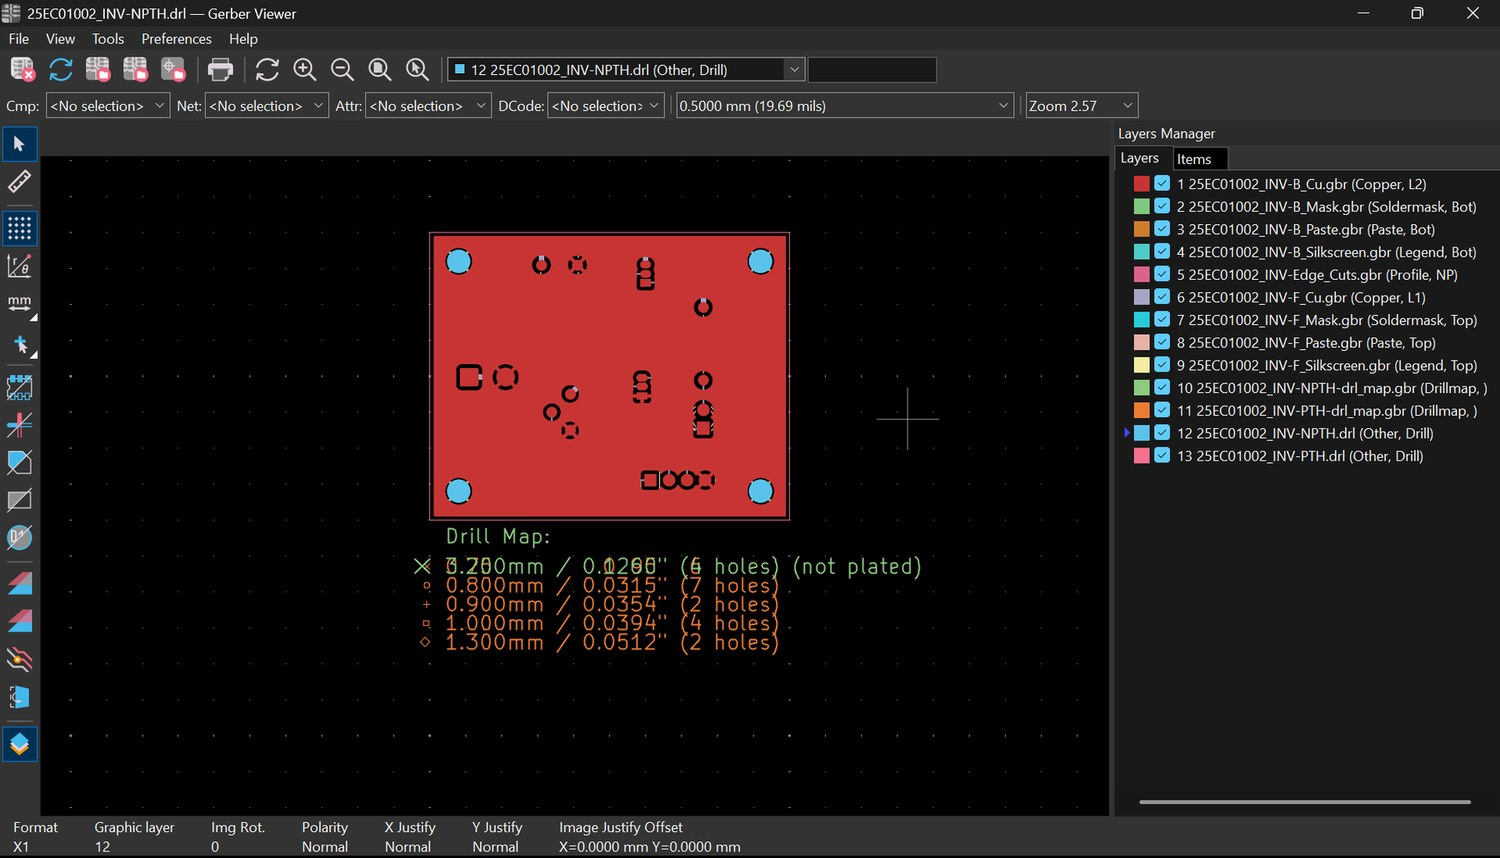
\includegraphics[width=0.84\linewidth]{figures/e5-gerbview.jpg}\caption{GerbView with the Exercise 5 Gerbers and drill files loaded.}\end{figure}

\lab{2.3}{What the change cost}
\begin{table}[H]\centering\small\sffamily
\begin{tabular}{@{}lcc@{}}\rowcolor{teal}\color{white}\textbf{Item}&\color{white}\textbf{Exercise 4}&\color{white}\textbf{Option 2}\\
Board size&50 $\times$ 40 mm&50 $\times$ 40 mm\\
\rowcolor{mist}Footprints moved&--&none\\
+5V copper (total)&102.9 mm&120.9 mm\\
\rowcolor{mist}VOUT copper&41.65 mm&41.20 mm\\
All tracks&214.5 mm (44 segments)&232.0 mm (47 segments)\\
\rowcolor{mist}+5V path, J1 to Q2&47.1 mm (0.028 $\Omega$)&47.1 mm (0.028 $\Omega$)\\\end{tabular}
\caption{Layout cost, measured from the two \texttt{.kicad\_pcb} files.}\end{table}
\begin{itemize}
\item Board area did not change and no part had to move, because the LED branch already sat beside R1; the cost is routing only.
\item R1's top end must now reach the +5V rail: \textbf{+17.95 mm} on +5V (+17 \%), while VOUT is 0.45 mm shorter. In total there is 17.5 mm more copper (+8 \%).
\item Parasitics: the extra 0.8 mm branch is about 12 m$\Omega$, i.e.\ 0.05 mV at 4.3 mA, negligible. The J1 to Q2 supply path is unchanged.
\end{itemize}
\begin{answer}
\textbf{Effect on the current drawn from the output node:}
\begin{itemize}
\item Exercise 4: with the output high, the PMOS \emph{sources} about 4.25 mA from VOUT into R1 and the LED; with the output low the load draws nothing.
\item Option 2: with the output high the LED branch draws \textbf{no current} from VOUT ($V_{OH}=5.00$ V, up from 4.94 V). With the output low, VOUT \emph{receives} 4.29 mA from +5 V through R1 and the LED, and the NMOS sinks it to ground.
\item The LED current is the same size but now flows through the 2N7000. Its effective on-resistance here is about 5 $\Omega$ (21 mV at 4.29 mA), against about 13 $\Omega$ (57 mV) for the BS250, so the output-low error is smaller than the earlier output-high droop.
\item $V_M$ rises from 2.35 V to 2.48 V. Near the transition the LED branch now pushes current into VOUT, which the NMOS must absorb, so it needs a larger $V_{IN}$; before, the PMOS had to supply the load, which pulled $V_M$ down.
\end{itemize}
\end{answer}

%------------------------------ OPTION 3
\lab{Option 3}{Minimum clearance raised to 0.4 mm}
\begin{itemize}
\item Change: Board Setup $\rightarrow$ clearance of the \texttt{Default} and \texttt{Power} net classes and the global minimum set from 0.2 mm to \textbf{0.4 mm}. Copper-to-edge distance stays 0.5 mm.
\item The circuit is unchanged, so no new simulation is needed: the electrical behaviour is the same as in Exercise 0.
\end{itemize}
\lab{3.1}{KiCad: rules, DRC and the fix}
\begin{figure}[H]\centering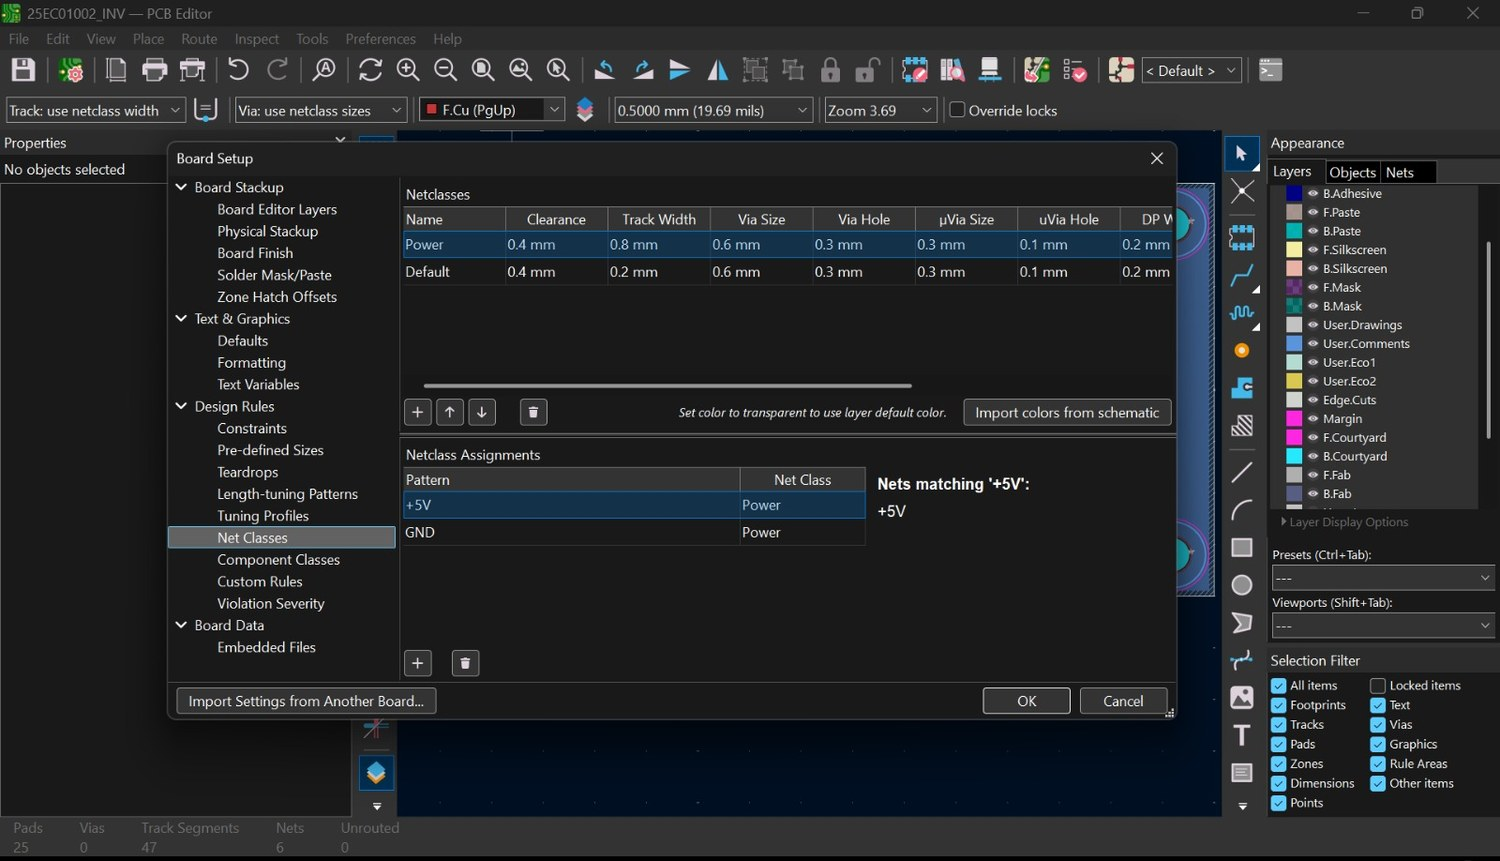
\includegraphics[width=0.66\linewidth]{figures/e5c-netclass.jpg}\caption{Net classes after the change: clearance 0.4 mm for \texttt{Power} (0.8 mm tracks) and \texttt{Default}.}\end{figure}
\begin{itemize}
\item First DRC run: \textbf{4 clearance errors}. Pads 1 and 2 of Q1 and of Q2 were only 0.227 mm apart against 0.4 mm required.
\item Cause: the \texttt{TO-92\_Inline} footprint has a 1.27 mm pad pitch with 1.05 mm wide pads, leaving a 0.22 mm gap. No routing can fix this, because both pads belong to the same footprint.
\item Fix: Q1 and Q2 changed to \texttt{TO-92\_Inline\_Wide} (2.54 mm pitch, 1.5 mm pads, \textbf{1.04 mm gap}). Pin numbers are unchanged, so the netlist is unchanged.
\item The tracks on +5V, VIN and VOUT around the transistors were re-routed and the ground pour refilled.
\end{itemize}
\begin{figure}[H]\centering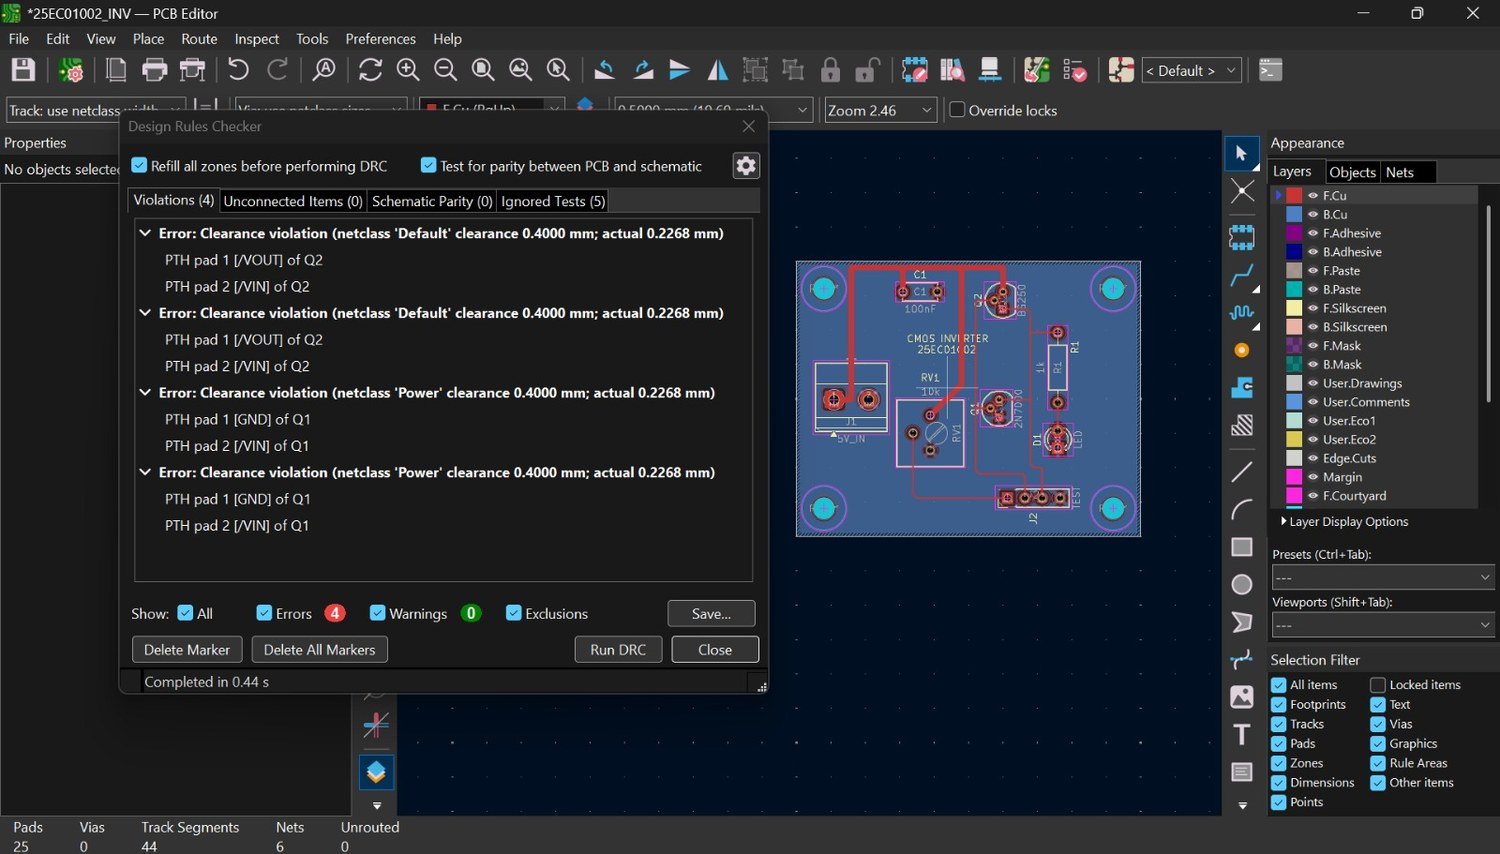
\includegraphics[width=0.7\linewidth]{figures/e5c-drc-before.jpg}\caption{DRC before the fix: 4 clearance violations at the transistor pads.}\end{figure}
\begin{figure}[H]\centering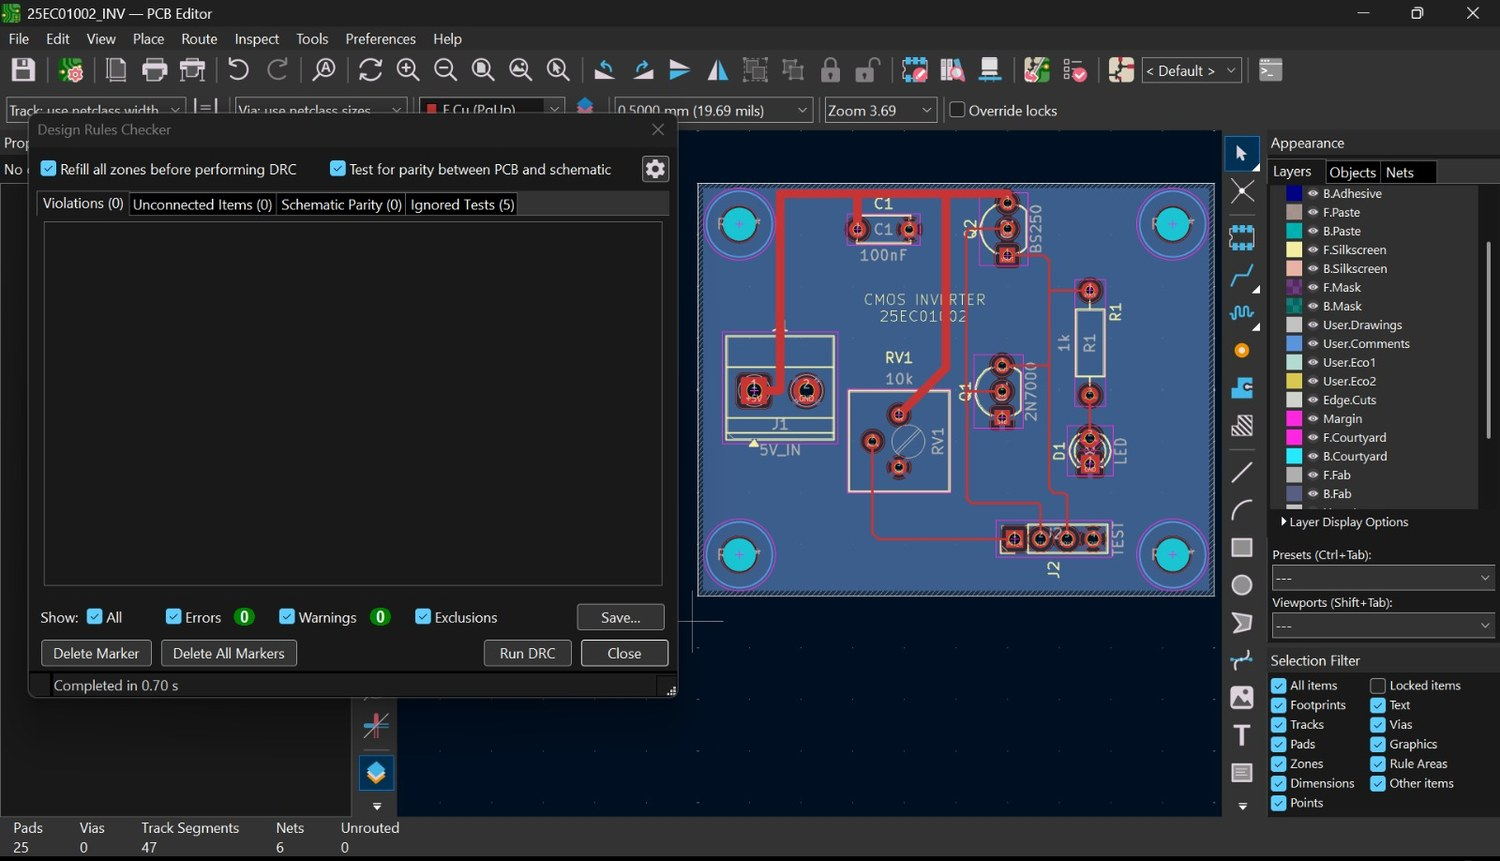
\includegraphics[width=0.84\linewidth]{figures/e5c-drc-after.jpg}\caption{DRC after the fix: Violations, Unconnected Items and Schematic Parity all 0 (47 track segments, 0 vias).}\end{figure}
\begin{itemize}
\item Gerbers and both drill files re-plotted to \texttt{gerbers\_ex5\_opt3/} and loaded back into GerbView (13 entries).
\end{itemize}
\begin{figure}[H]\centering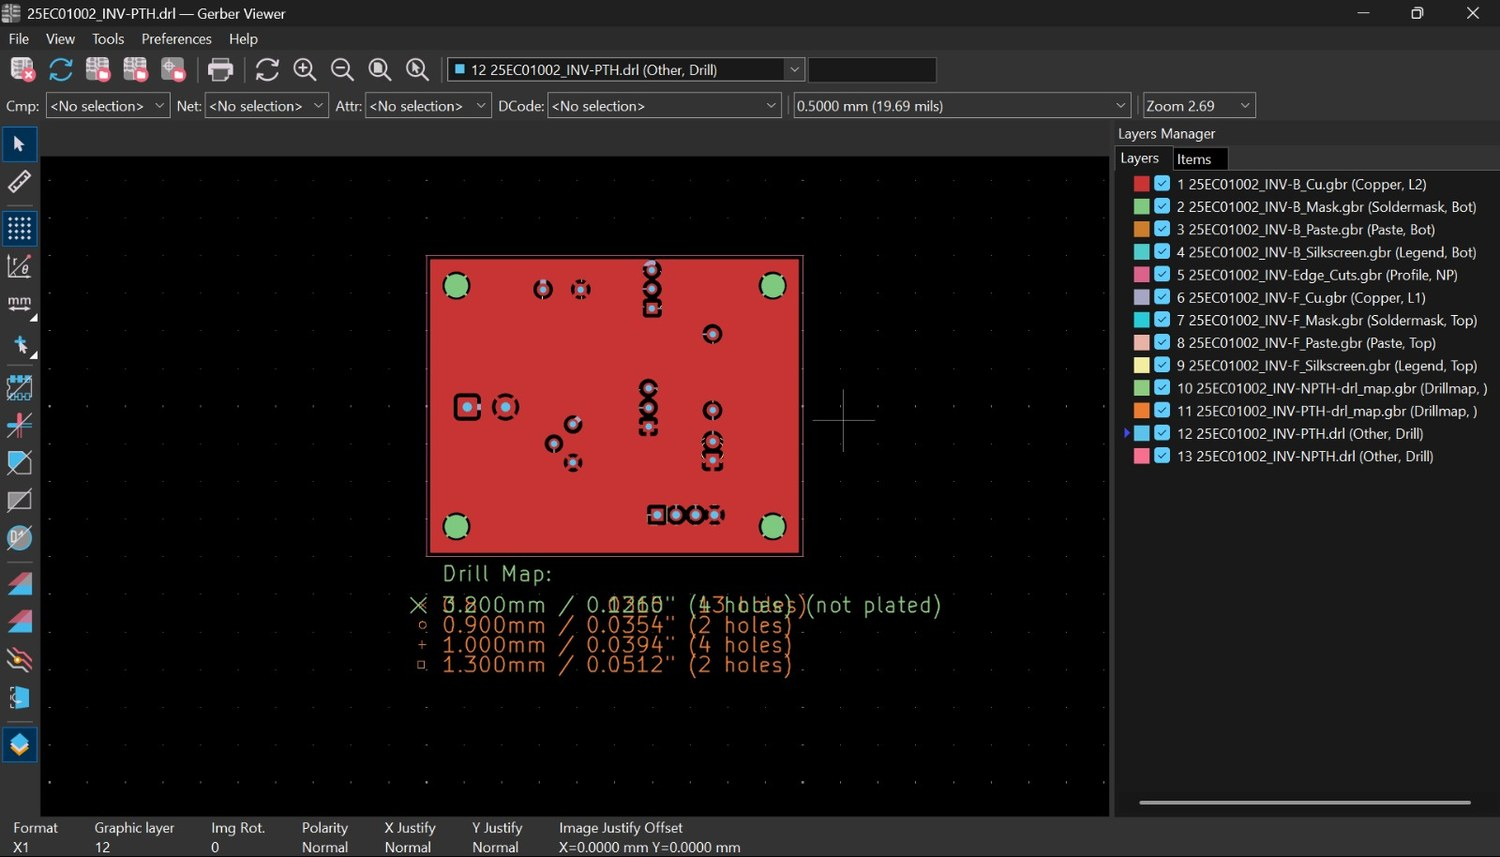
\includegraphics[width=0.8\linewidth]{figures/e5c-gerbview.jpg}\caption{GerbView with the option 3 Gerbers and drill files loaded.}\end{figure}
\Needspace{18\baselineskip}
\lab{3.2}{What the change cost}
\begin{table}[H]\centering\small\sffamily
\begin{tabular}{@{}lcc@{}}\rowcolor{teal}\color{white}\textbf{Item}&\color{white}\textbf{Exercise 4}&\color{white}\textbf{Option 3}\\
Board size&50 $\times$ 40 mm&50 $\times$ 40 mm\\
\rowcolor{mist}Footprints moved&--&none (positions unchanged)\\
Footprints changed&--&Q1, Q2: pitch 1.27 $\rightarrow$ 2.54 mm\\
\rowcolor{mist}Pad gap, Q1/Q2 pads 1--2&0.22 mm&1.04 mm\\
+5V copper&102.9 mm&100.4 mm\\
\rowcolor{mist}VIN copper&42.9 mm&44.3 mm\\
VOUT copper&41.65 mm&41.64 mm\\
\rowcolor{mist}All tracks&214.5 mm (44 segments)&213.3 mm (47 segments)\\
Vias&0&0\\
\rowcolor{mist}Q2 drain (A) to Q1 drain (B), straight line&13.20 mm&10.66 mm\\
J1 pin 1 (C) to Q2 source (D), straight line&29.12 mm&30.56 mm\\\end{tabular}
\caption{Layout cost of option 3, measured from the two \texttt{.kicad\_pcb} files.}\end{table}
\begin{answer}
\textbf{What it cost:}
\begin{itemize}
\item Board area did not change and no part had to move; only Q1 and Q2 changed footprint (each now 2.54 mm longer) and the tracks around them were re-routed.
\item Total copper is 1.2 mm shorter (--0.6 \%); VIN is 1.4 mm longer, +5V is 2.5 mm shorter, and the A--B drain link is 2.5 mm shorter, so parasitics are practically unchanged.
\item On the real parts, the outer leads of each TO-92 must be splayed to fit the 2.54 mm pads, a small assembly cost.
\item A 0.4 mm rule is only met here because of the wider footprint: with the original pads, 0.4 mm clearance could not be reached at all.
\end{itemize}
\end{answer}

\lab{Option 4}{Trimpot replaced by a 2-pin header, board shrunk}
\begin{itemize}
\item Change: RV1 and the \texttt{POT\_W} net removed; a 2-pin header \textbf{J3} added (pin 1 = VIN, pin 2 = GND) so the input comes only from outside; J2 became a 3-pin test header (VIN, VOUT, GND). Then the board was shrunk until the DRC was still clean.
\item Simulation: the circuit already uses an external $V_{IN}$ source in LTspice (Exercise 0), so the results are unchanged; the trimpot divider (about 0.5 mA at 5 V) is no longer drawn from the supply.
\item DRC: \textbf{0 violations, 0 unconnected items, 0 schematic-parity errors} (23 pads, 5 nets, 26 track segments, 0 vias).
\end{itemize}
\begin{figure}[H]\centering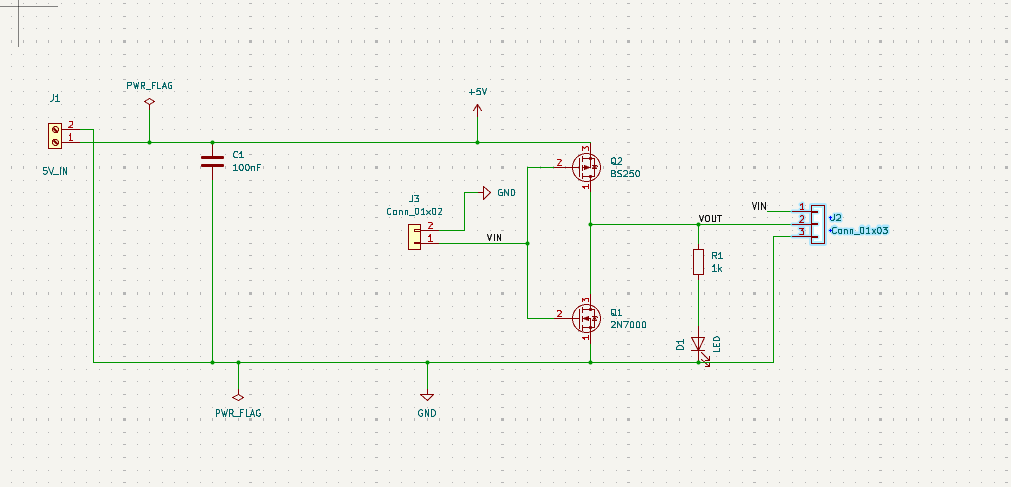
\includegraphics[width=0.9\linewidth]{figures/e5o4-schematic.png}\caption{Option 4 schematic: J3 supplies VIN and GND; RV1 and POT\_W removed; J2 has VIN, VOUT and GND.}\end{figure}
\begin{figure}[H]\centering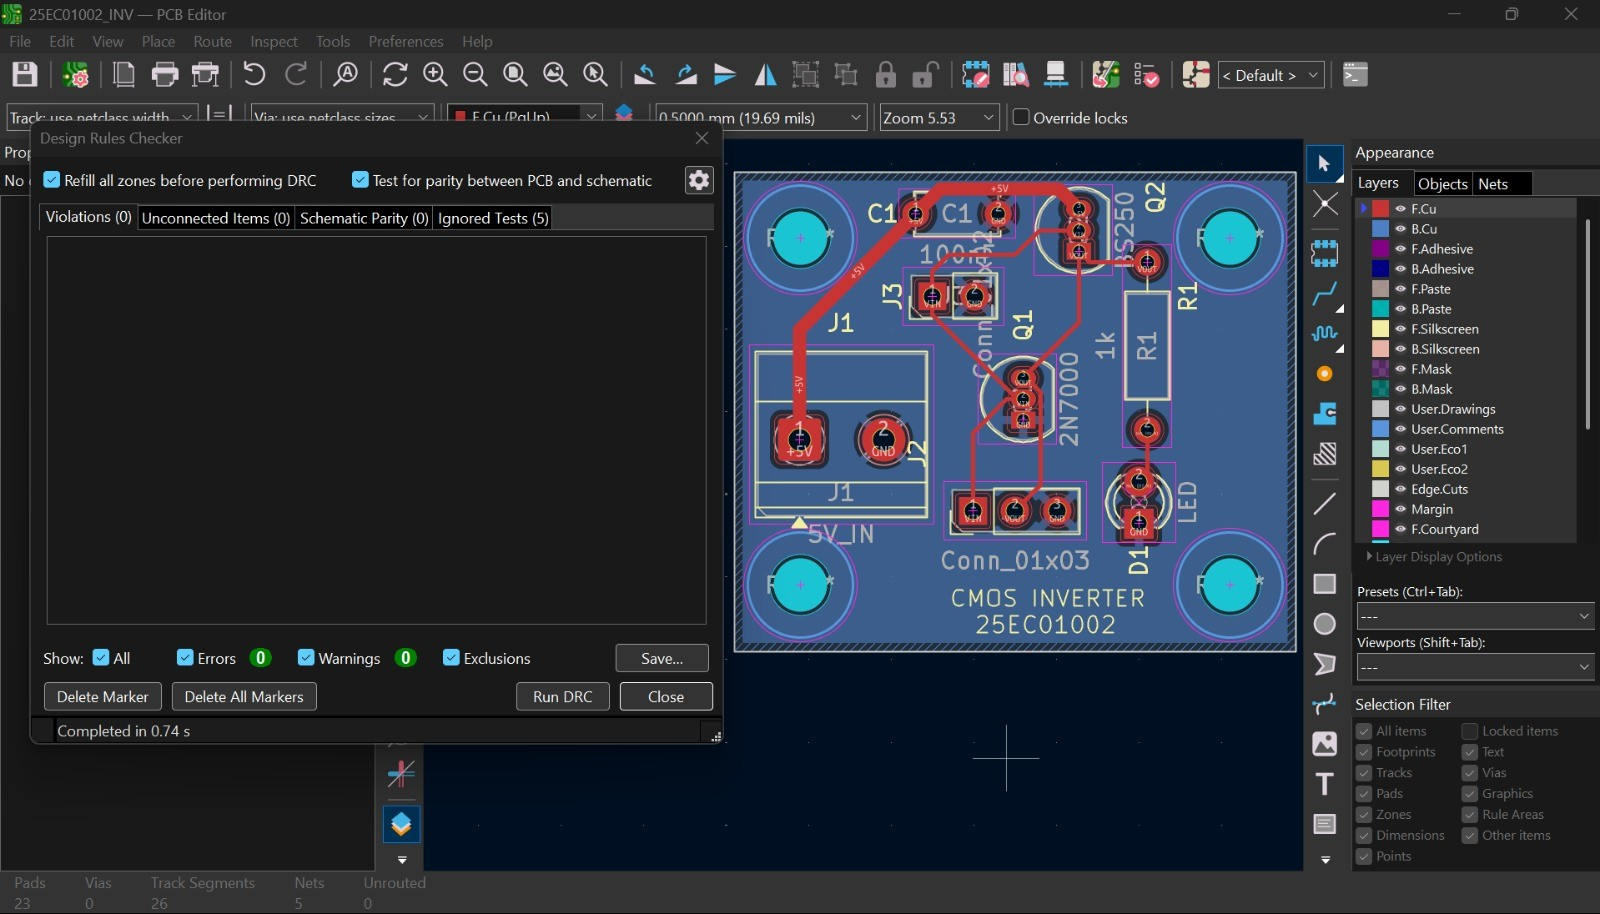
\includegraphics[width=0.84\linewidth]{figures/e5o4-drc.jpg}\caption{Shrunk board with the DRC clean: Violations, Unconnected Items and Schematic Parity all 0.}\end{figure}
\begin{figure}[H]\centering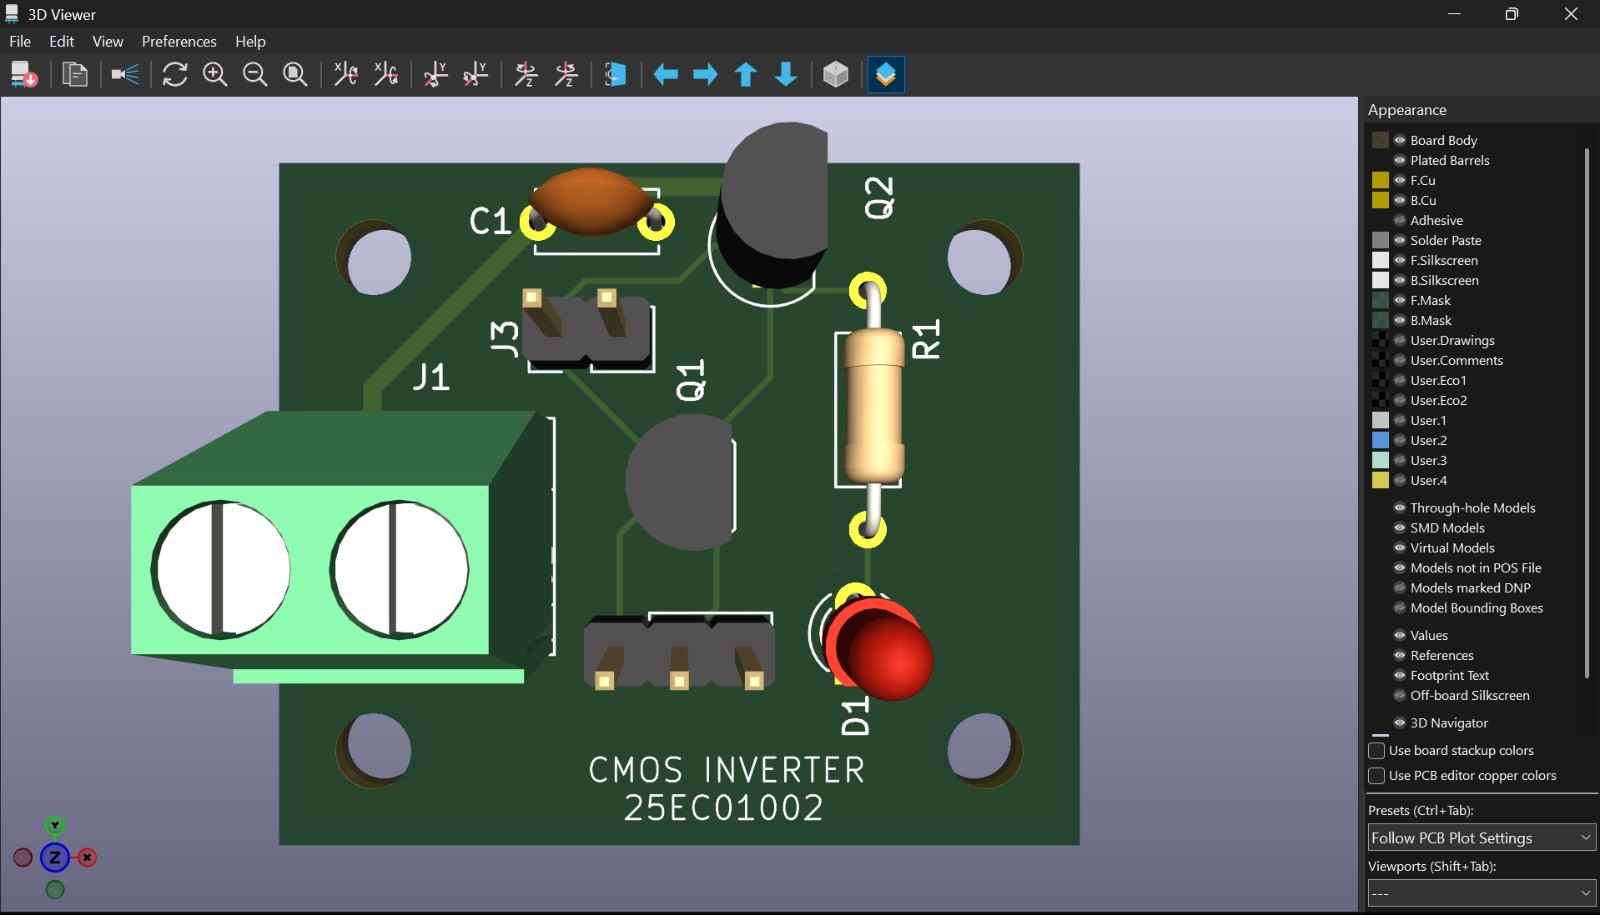
\includegraphics[width=0.84\linewidth]{figures/e5o4-3d.jpg}\caption{3D viewer, top of the shrunk board (J3 header, J2 test header).}\end{figure}
\begin{figure}[H]\centering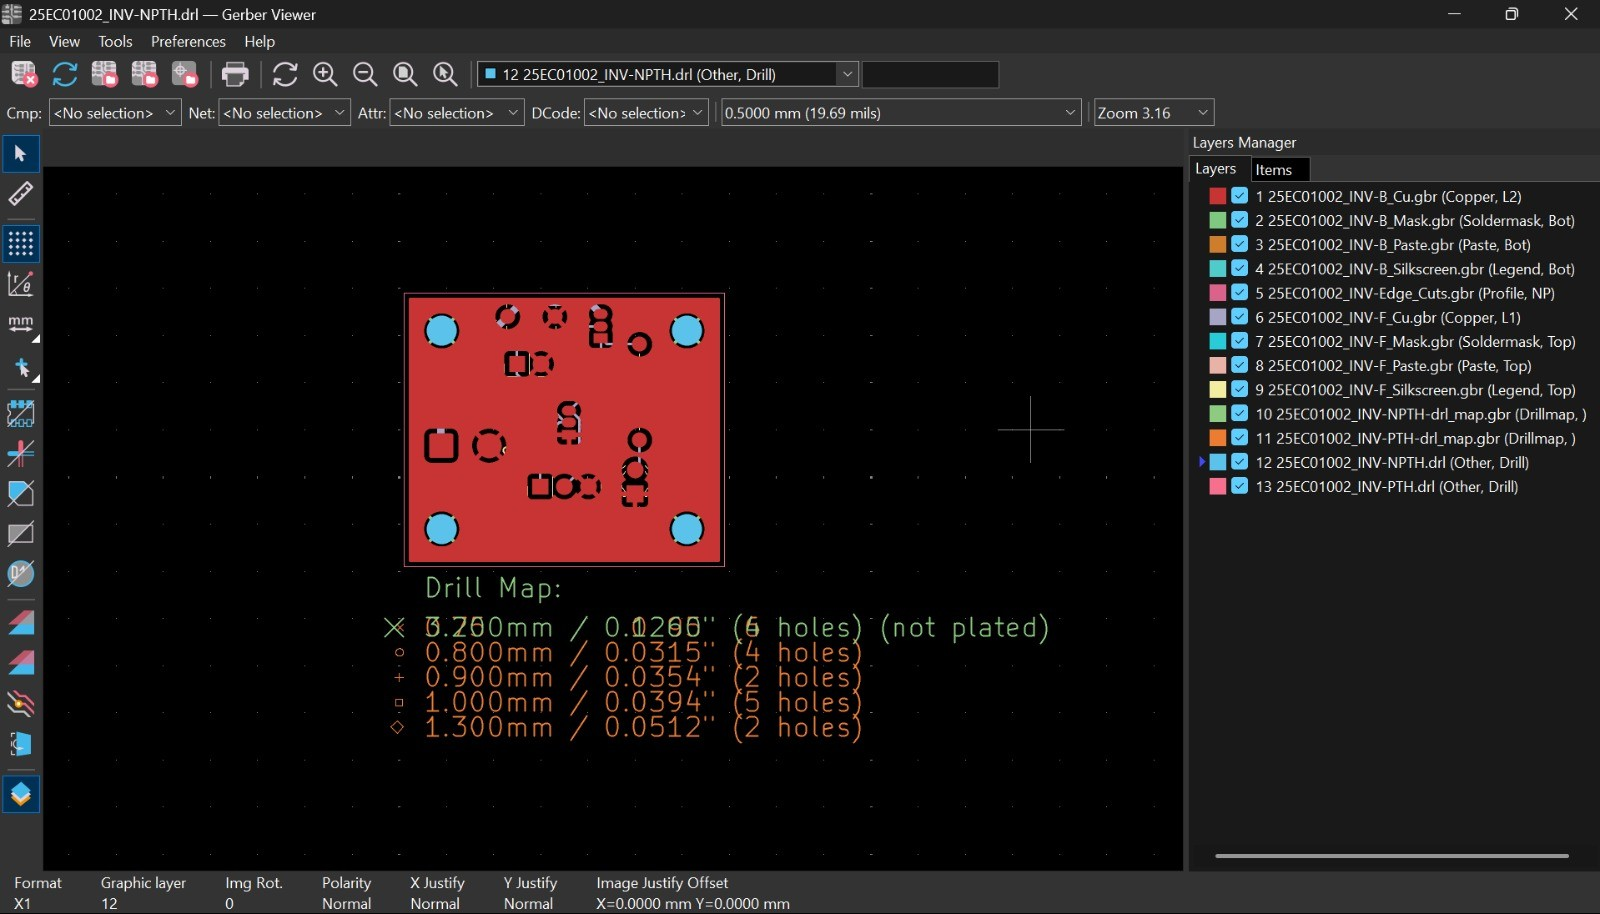
\includegraphics[width=0.84\linewidth]{figures/e5o4-gerbview.jpg}\caption{GerbView with the option 4 Gerbers and drill files loaded (13 entries).}\end{figure}
\Needspace{20\baselineskip}
\begin{table}[H]\centering\small\sffamily
\begin{tabular}{@{}lcc@{}}\rowcolor{teal}\color{white}\textbf{Item}&\color{white}\textbf{Exercise 4}&\color{white}\textbf{Option 4}\\
Board size&50 $\times$ 40 mm&34 $\times$ 29 mm\\
\rowcolor{mist}Board area&2000 mm$^2$&986 mm$^2$ ($-50.7$ \%)\\
Parts&8 (RV1, 4-pin J2)&8 (J3 added, RV1 removed, 3-pin J2)\\
\rowcolor{mist}Pads / nets&25 / 6&23 / 5\\
Footprints moved&--&all remaining parts re-placed\\
\rowcolor{mist}+5V copper&102.9 mm&27.6 mm\\
VIN copper&42.9 mm&28.7 mm\\
\rowcolor{mist}VOUT copper&41.65 mm&22.8 mm\\
POT\_W copper&22.9 mm&removed\\
\rowcolor{mist}All tracks&214.5 mm (44 segments)&82.4 mm (26 segments)\\
Vias&0&0\\
\rowcolor{mist}J1 pin 1 (A) to Q2 source (B), straight line&29.12 mm&21.91 mm\\
Q2 drain (C) to Q1 drain (D), straight line&13.20 mm&8.39 mm\\\end{tabular}
\caption{Layout cost of option 4, measured from the two \texttt{.kicad\_pcb} files.}\end{table}
\begin{answer}
\textbf{What it cost and gained:}
\begin{itemize}
\item Board area fell by half (2000 $\to$ 986 mm$^2$) and total copper by 62 \% (214.5 $\to$ 82.4 mm), so track resistance and parasitics are lower; the A--B supply link is 7.2 mm shorter and the C--D drain link 4.8 mm shorter.
\item Removing the trimpot also removed the POT\_W net and one test-header pin, and saves the 0.5 mA divider current.
\item Cost: every part had to be re-placed and re-routed, and the four M3 holes were moved to stay exactly 4 mm from the new corners. The board is tighter to solder and probe, and VIN can no longer be adjusted on the board itself.
\end{itemize}
\end{answer}

\Needspace{16\baselineskip}
\lab{Summary}{All four options against Exercise 4}
\begin{table}[H]\centering\small\sffamily
\begin{tabular}{@{}llccc@{}}\rowcolor{teal}\color{white}\textbf{Design}&\color{white}\textbf{Change}&\color{white}\textbf{Board}&\color{white}\textbf{Copper}&\color{white}\textbf{DRC}\\
Exercise 4&--&50 $\times$ 40 mm&214.5 mm&0 / 0 / 0\\
\rowcolor{mist}Option 1&second stage (buffer)&50 $\times$ 40 mm&253.9 mm&0 / 0 / 0\\
Option 2&LED lights when output low&50 $\times$ 40 mm&232.0 mm&0 / 0 / 0\\
\rowcolor{mist}Option 3&clearance 0.4 mm&50 $\times$ 40 mm&213.3 mm&0 / 0 / 0\\
Option 4&header instead of trimpot&34 $\times$ 29 mm&82.4 mm&0 / 0 / 0\\\end{tabular}
\caption{Exercise 5 summary: board size, total track length and DRC result (violations / unconnected / parity).}\end{table}
\begin{itemize}
\item Options 1, 2 and 3 cost only routing (and two moved parts in option 1), because the board outline stayed the same. Option 4 is the only one that changes the board area, and it gains space but loses the on-board input adjustment.
\item Option 1 adds the most copper (+18 \%) and fills the free right-hand side of the board.
\item Option 3 shows that a stricter fabricator rule can force a different component footprint, not just more careful routing.
\end{itemize}

%------------------------------------------------------------ END
\exhead{Conclusions}{Overall observations}
\begin{itemize}
\item Simulation vs.\ board: expect $V_M\approx2.35$ V, $V_{OH}\approx4.94$ V, $V_{OL}\approx0$ V; LED on below about 2.3 V, off above about 2.5 V; check $V_{IN}$ and $V_{OUT}$ at J2.
\item Simulating first gives target numbers ($V_M$, levels, LED current) to test the real board against.
\item Clean ERC/DRC shows consistency and manufacturability, not correct behaviour; lead order and polarity must be checked against datasheets.
\item Track width was electrically irrelevant at milliamps (28 m$\Omega$ path); clearance, edge distance and complete files decide manufacturability.
\item Exercise 5 (optional): all four options were done, each on its own copy of the Exercise 4 project.
\begin{itemize}
\item \textbf{Option 1, second inverter stage (buffer):} the output follows the input ($V_M$ 2.415 V, delay 16 ns, of which 4.9 ns is stage 1). The 50 $\times$ 40 mm board still fits after moving only R1 and D1 by 7.5 mm; copper grew by 39.4 mm (+18 \%) and the longest new supply path is 55.7 mm.
\item \textbf{Option 2, LED lights when the output is low:} the board stayed 50 $\times$ 40 mm and 17.5 mm of copper was added (+8 \%). $V_M$ moved from 2.35 V to 2.48 V, and the LED current stayed near 4.3 mA but now flows through the NMOS.
\item \textbf{Option 3, clearance raised to 0.4 mm:} the TO-92 pads of Q1 and Q2 were too close, so both parts needed the wider footprint and the tracks around them were re-routed. The board stayed 50 $\times$ 40 mm, no part moved and total copper fell by 1.2 mm.
\item \textbf{Option 4, trimpot replaced by a header:} the board shrank to 34 $\times$ 29 mm (half the area) with 62 \% less copper, at the price of needing an external input source.
\end{itemize}
\end{itemize}

\end{document}
